%%%%%%%%%%%%%%%%%%%%%%%%%%%%%%%%%%%%%%%%%%%%%%%%%%%%%%%%%%%%%%%%%%%%%%%%%%%%%%%%
%%%%%%%%%%%%%%%%%%   Vorlage für eine Abschlussarbeit   %%%%%%%%%%%%%%%%%%%%%%%%
%%%%%%%%%%%%%%%%%%%%%%%%%%%%%%%%%%%%%%%%%%%%%%%%%%%%%%%%%%%%%%%%%%%%%%%%%%%%%%%%

% Erstellt von Maximilian Nöthe, <maximilian.noethe@tu-dortmund.de>
% ausgelegt für lualatex und Biblatex mit biber

% Kompilieren mit 
% lualatex dateiname.tex
% biber dateiname.bcf
% lualatex dateiname.tex
% lualatex dateiname.tex
% oder einfach mit:
% make

\documentclass[
  BCOR=12mm,     % 12mm binding corrections, adjust to fit your binding
  parskip=half,  % new paragraphs start with half line vertical space
  open=any,      % chapters start on both odd and even pages
  cleardoublepage=plain,  % no header/footer on blank pages
]{tudothesis}


% Warning, if another latex run is needed
\usepackage[aux]{rerunfilecheck}

% just list chapters, sections and subsections in the toc, not subsubsection or smaller
\setcounter{tocdepth}{2}

%------------------------------------------------------------------------------
%------------------------------ Sprache und Schrift: --------------------------
%------------------------------------------------------------------------------
\usepackage{fontspec}
\defaultfontfeatures{Ligatures=TeX}  % -- becomes en-dash etc.

% german language
\usepackage{polyglossia}
\setdefaultlanguage{german}

% for english abstract and english titles in the toc
\setotherlanguages{english}

% intelligent quotation marks, language and nesting sensitive
\usepackage[autostyle]{csquotes}

% microtypographical features, makes the text look nicer on the small scale
\usepackage{microtype}

%------------------------------------------------------------------------------
%------------------------ Für die Matheumgebung--------------------------------
%------------------------------------------------------------------------------

\usepackage{amsmath}
\usepackage{amssymb}
\usepackage{mathtools}
\usepackage{upgreek}

% Enable Unicode-Math and follow the ISO-Standards for typesetting math
\usepackage[
  math-style=ISO,
  bold-style=ISO,
  sans-style=italic,
  nabla=upright,
  partial=upright,
]{unicode-math}
\setmathfont{Latin Modern Math}

% nice, small fracs for the text with \sfrac{}{}
\usepackage{xfrac}  


%------------------------------------------------------------------------------
%---------------------------- Numbers and Units -------------------------------
%------------------------------------------------------------------------------

\usepackage[
  locale=DE,
  separate-uncertainty=true,
  output-decimal-marker = {.},
  per-mode=symbol-or-fraction,
]{siunitx}
\sisetup{math-micro=\text{µ},text-micro=µ}

%------------------------------------------------------------------------------
%-------------------------------- tables  -------------------------------------
%------------------------------------------------------------------------------

\usepackage{booktabs}       % stellt \toprule, \midrule, \bottomrule

%------------------------------------------------------------------------------
%-------------------------------- graphics -------------------------------------
%------------------------------------------------------------------------------

\usepackage{graphicx}
\usepackage{grffile}

% allow figures to be placed in the running text by default:
\usepackage{scrhack}
\usepackage{float}
\floatplacement{figure}{htbp}
\floatplacement{table}{htbp}

% keep figures and tables in the section
\usepackage[section, below]{placeins}


%------------------------------------------------------------------------------
%---------------------- customize list environments ---------------------------
%------------------------------------------------------------------------------

\usepackage{enumitem}

%------------------------------------------------------------------------------
%------------------------------ Bibliographie ---------------------------------
%------------------------------------------------------------------------------

\usepackage[
backend=biber,   % use modern biber backend
autolang=hyphen, % load hyphenation rules for if language of bibentry is not
% german, has to be loaded with \setotherlanguages
% in the references.bib use langid={en} for english sources
bibstyle=phys_msc,
citestyle=phys_msc,
sorting=nyt
%style=phys
]{biblatex}
\addbibresource{references.bib}  % die Bibliographie einbinden
\DefineBibliographyStrings{german}{andothers = {{et\,al\adddot}}} 

%------------------------------------------------------------------------------
%------------------------------ Sonstiges: ------------------------------------
%------------------------------------------------------------------------------

\usepackage[pdfusetitle,unicode,linkbordercolor=tugreen]{hyperref}
\usepackage{bookmark}
\usepackage[shortcuts]{extdash}

\usepackage{listings}

\lstset{
	breaklines=true,
%	postbreak=\raisebox{0ex}[0ex][0ex]{\ensuremath{\color{red}\hookrightarrow\space}}
}

\usepackage{chemformula}


% Custom

\usepackage{rotating}
% \usepackage{mwe}
% \usepackage{subfig}
% \usepackage{lscape}

\newcommand*\circled[1]{\tikz[baseline=(char.base)]{
    \node[shape=circle,draw,inner sep=1pt] (char) {#1};}}

\newcommand{\myvec}[1]{\ensuremath{\begin{pmatrix}#1\end{pmatrix}}}
\usepackage{braket}

\usepackage{wrapfig}

%------------------------------------------------------------------------------
%-------------------------    Angaben zur Arbeit   ----------------------------
%------------------------------------------------------------------------------

\author{Jens Adam}
\title{$^\text{87}$Rb-NMR Untersuchungen an Calciumrubidiumnitrat:\\Experiment und Simulation}
\date{2018}
\birthplace{Bielefeld}
\chair{Lehrstuhl für Experimentelle Physik III}
\division{Fakultät Physik}
\thesisclass{Master of Science}
\submissiondate{23. April 2018}
\firstcorrector{Prof.~Dr.~Roland~Böhmer}
\secondcorrector{Priv.-Doz.~Dr.~Ute~Löw}

% tu logo on top of the titlepage
\titlehead{\includegraphics[height=1.5cm]{logos/tu-logo.pdf}}

\begin{document}
\frontmatter
\maketitle

% Gutachterseite
\makecorrectorpage

% hier beginnt der Vorspann, nummeriert in römischen Zahlen
%\input{content/00_abstract.tex}
\tableofcontents

\mainmatter
% Hier beginnt der Inhalt mit Seite 1 in arabischen Ziffern
\chapter{Einleitung}


Durch den immer weiter fortschreitenden Umstieg auf erneuerbare Energien, werden gute Möglichkeiten zur Speicherung der gewonnenen Energie zunehmend wichtiger -- dies resultiert in einem entsprechend hohen Forschungsinteresse. Ein Vorschlag für eine neue Technologie ist die Nutzung von ionische Flüssigkeiten. Um aber am Ende effiziente Produkte herstellen zu können, müssen die physikalischen Vorgänge auf mikroskopischer Ebene verstanden sein. Dies betrifft insbesondere die Struktur und Dynamik von Molekülen und Atomen. 

Dafür kann die magnetische Kernspinresonanz (kurz NMR vom engl. „magnetic nuclear resonance“) eine hilfreiche Methode sein, ist sie doch beispielsweise für die Auflösung von Strukturen ein allgegenwärtig verwendetes Werkzeug von Chemikern. Aber auch die Möglichkeit, die Untersuchung auf ein bestimmtes Isotop zu beschränken, macht es möglich, den Einfluss der Dynamik von verschiedenen Komponenten eines Moleküls separat zu untersuchen.

In dieser Arbeit wurde Calciumrubidiumnitrat, kurz CRN, mit $^\text{87}$Rb-NMR untersucht. Dabei handelt es sich um ein Nitratsalz, welches bei entsprechend schnellem Abkühlen ein Glas, also einen amorphen Feststoff, bildet. Vorhergegangene Untersuchungen von CRN umfassen unter anderem die Untersuchungen von C. Zürn, welcher sich ebenfalls $^\text{87}$Rb-NMR beschäftigt hat \cite{zuern_paper} und auf dessen Ergebnisse diese Arbeit teilweise aufbaut.
\begin{figure}
	\begin{center}
		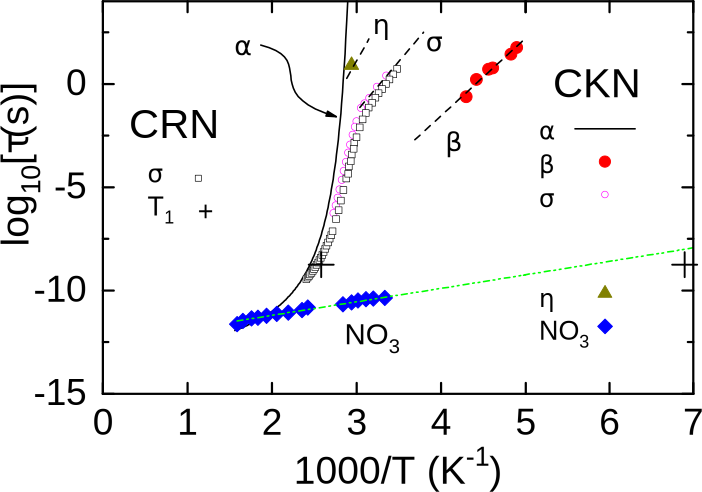
\includegraphics[width=.7\textwidth]{graphics/zuern/Plot1_b.pdf}
	\end{center}
	\caption{Relaxationskarte aus \cite{zuern_paper}, dargestellt in einem Arrhenius-Diagramm (logarithmierte Zeitkonstanten aufgetragen gegen die inverse Temperatur). Gezeigt sind ermittelte Zeitkonstanten aus Untersuchungen an CRN und CKN. Hierbei sind für diese Arbeit insbesondere der Betaprozess, dargestellt in rot, interessant. Die Daten hierzu stammen aus \cite{}} \label{fig:einl:zuernpaper}
\end{figure}

Eine Graph aus dem erwähnten Paper ist in Abbildung \ref{fig:einl:zuernpaper} zu sehen. Hier sind in CKN, kurz für Calciumkaliumnitrat, entdeckte Hinweise auf einen Betaprozess, dargestellt in rot, hervorzuheben. Die gestrichelte Linie durch die Punkte zeigt die lineare Fortsetzung der Punkte im Arrhenius-Diagramm an. Sollte dieser Trend standhalten, sollten bei Temperaturen in Bereichen kurz unter oder bei der Glasübergangstemperatur von $T_g = \SI{333}{K}$ Zeitkonstanten im hohen Mikrosekunden-Bereich zu erwarten sein. Zeitkonstanten dieser Größenordnungen lassen sich mit Methoden der NMR -- zum Beispiel der hier verwendeten Untersuchung von stimulierten Echos oder der Analyse von Linienformen von pulslängenabhängigen Spektren -- gut untersuchen.

Die Stoffe CKN und CRN ähneln sich sehr. Bis auf das gegen ein Rubidium-Atom ausgetauschte Kalium-Atom, welches der gleichen Hauptgruppe entstammt, teilen sie die gleiche Struktur, Glasübergangstemperatur und weitere Eigenschaften \cite{PIMENOV199793}. So ist beispielsweise auch in Abbildung \ref{fig:einl:zuernpaper} die Übereinstimmung von Leitfähigkeitsdaten $\sigma$ zwischen CRN und CKN zu erkennen. Daher ist es nachvollziehbar, für CRN und CKN ähnliche Zeitkonstanten eines Betaprozesses zu erwarten.

Während dieser Messungen wurde entdeckt, dass die Halbwertsbreite von CRN-Spektren zu höheren Temperaturen erst abnimmt -- was aufgrund der ansteigenden Bewegungsverschmälerung zu höheren Temperaturen zu erwarten ist -- aber bei Temperaturen ab $\SI{375}{K}$ wieder zunimmt. Dies widerspricht der naiven Erwartung, dass die Halbwertsbreite zu steigenden Temperaturen in diesem Fall lediglich abnehmen sollte. Um die Gründe dieses Phänomen zu klären wurden Spektren simuliert und ein Vergleich mit der Theorie der Quadrupol-Wechselwirkung zweiter Ordnung, welche hier entscheidende Einflüsse hat, durchgeführt.


Zunächst sollen in Kapitel \ref{chapter:theo} die theoretischen Grundlagen der NMR erläutert werden und eine Einführung in die Relaxation der Quadrupol-Wechselwirkung zweiter Ordnung gegeben werden. Kapitel \ref{chapter:simulation} beschreibt die für die Simulation verwendete Software mit zugehörigem Bewegungsmodell. Außerdem wird ein weiteres Bewegungsmodell vorgestellt, in der Zukunft facettiertere Untersuchungen ermöglichen könnte. In Kapitel \ref{chapter:exp_details} die verwendeten Apparaturen und Proben beschrieben, ehe in Kapitel \ref{chapter:experiment} die aufgenommenen Daten zunächst gezeigt, und dann ausgewertet und analysiert werden. Eine Zusammenfassung der Ergebnisse und ein Ausblick auf mögliche zukünftige Untersuchungen bilden den Abschluss der Arbeit.

\chapter{Theoretische Einführung}
\label{ch:theo}

\chapter{Simulation}\label{chapter:simulation}

Simulationen werden in vielen Disziplinen der Physik gerne verwendet, da sie es ermöglichen, Sachverhalte schnell, flexibel und kostengünstig zu untersuchen. Weiter können die Grenzen des experimentell Realisierbaren überschritten werden, da diese Grenzen in der simulierten Umgebung nicht zwingend existieren müssen.

Auf der Gegenseite müssen sich Simulationen, die ein Experiment wie die NMR-Spektroskopie nachstellen, meist auf eine Auswahl der unter Laborbedingungen vorliegenden Einflüsse und Wechselwirkungen beschränken. Zu groß ist die Zahl der (teilweise auch unbekannten) Parameter. Eine Simulation kann also in der Regel nur als eine Näherung eines Experiments verstanden werden.

Aber gerade wegen der geringeren Zahl der Parameter einer Simulation ist der Vergleich von Simulation und Experiment von besonderer Bedeutung. Soll zum Beispiel untersucht werden, ob eine bestimmte gemessene Eigenschaft durch eine bestimmte Wechselwirkung hervorgerufen wird, kann eine entsprechende Simulation durchgeführt werden, wobei bei dieser die Zahl der möglichen Einflüsse deutlich reduziert werden kann -- andere Wechselwirkungen als die von Interesse müssen nicht simuliert werden. Ein Vergleich der simulierten Eigenschaften mit den gemessenen kann dann einen bestehenden Verdacht bestärken oder entkräften, je nach dem, inwiefern sich Experiment und Simulation ähneln.


Aus diesen Gründen wurde an diesem Lehrstuhl eine Simulationssoftware von J. Beerwerth in der Programmiersprache C++ geschrieben, aktiv weiterentwickelt, und beispielsweise in \cite{joachim_master} verwendet. Dabei handelt es sich um eine Random-Walk-Simulation. Diese soll NMR-Experimente simulieren und beinhaltet eine Vielzahl von Möglichkeiten. Während nicht jeder Teil der Simulationssoftware explizit benannt werden soll, soll dennoch der Aufbau nachvollzogen werden, um eine Einschätzung ihrer Möglichkeiten bieten zu können. Jede Simulation besteht aus drei Komponenten, die unabhängig von einander gewählt werden können: Die Art der Messung (beispielsweise ein 2D-Spektrum, Hahn-Echo oder ein stimuliertes Echo), das Bewegungsmodell (zum Beispiel Sprünge zwischen $N$ festen Plätzen oder ein isotroper Sprung) und die zu berücksichtigen Wechselwirkungen (wie die Quadrupol-Wechselwirkung erster oder zweiter Ordnung, oder die chemische Verschiebung).

Die Software ist modular aufgebaut, um Erweiterungen, beispielsweise einer anderen Wechselwirkung, leicht zuzulassen. Dazu werden die drei Komponenten, die Wechselwirkung, das Bewegungsmodell, und die Art der Messung, mit Hilfe von abstrakten Klassen implementiert. Diese lauten \texttt{Frequency}, \texttt{MotionalModel}, und \texttt{Measurement}. Zum Hinzufügen zusätzlicher Wechselwirkungen muss von der entsprechenden abstrakten Klasse \texttt{Frequency} geerbt werden, um sie anstelle einer anderen Wechselwirkung verwenden zu können. Die Klasse \texttt{NMRSimulation} bildet das Herzstück der Software. Per Komandozeile übergebene Parameter werden geparst und gespeichert oder an die richtigen Klassen weitergeleitet, und die eigentliche Simulation dann gestartet.

Die Arbeitsweise der Software soll an den drei Komponenten verdeutlicht werden, die für diese Arbeit verwendet wurden: Die FID-Pulsfolge, die Quadrupol-Wechselwirkung zweiter Ordnung, und das Bewegungsmodell des isotropen Sprungs. Es muss betont werden, dass folgende Beschreibung auf Verständlichkeit ausgelegt ist und nicht den tatsächlichen Programmablauf korrekt wiedergibt. Die grundlegenden Abläufe und Ideen sind aber identisch.

Mit Hilfe der Simulation soll beobachtet werden, wie ein simulierter Kern eine Reihe von Sprüngen durchläuft, welche jeweils in einer unterschiedlichen Ladungsumgebung resultieren. Der Kern verbleibt für eine bestimmte Zeit, der sogenannten Lebenszeit, in jeder dieser Umgebungen. Die Lebenszeit wird zufällig aus einer Exponentialverteilung gezogen. Da mit steigender Temperatur in der Regel die Bewegung, und damit auch die Anzahl der Sprünge steigt, kann über diesen Parameter eine Verknüpfung zu Temperaturen hergestellt werden. Dazu können zum Beispiel Korrelationszeiten wie aus Gleichung \eqref{eqn:theo:tauc} verwendet werden.

Ist die Lebenszeit vergangen, wird ein neuer Sprung mit einer neuen Lebenszeit durchgeführt. So reiht sich eine Kette von Umgebungen, jede mit ihrer eigenen Dauer, aneinander. Dies wird so lange durchgeführt, bis das Ende der zu simulierenden Zeit erreicht ist. Diese bestimmt sich aus der Anzahl der aufzunehmenden Datenpunkte multipliziert mit dem Zeitabstand zwischen zwei Datenpunkten, genannt dwelltime.

In diesem Fall handelt es sich bei den erwähnten Sprüngen um isotrope Sprünge in Kombination mit dem Czjzek-Modell \cite{czjzek_atomic_1981}. Das Czjzek-Modell kann für Gläser oder ähnliche amorphe Stoffe angewandt werden, in dem die Ladungsverteilung nicht, wie beispielsweise durch ein Gitter, periodisch, sondern annähernd isotrop ist. Die aus den entsprechenden Ladungsverteilungen resultierenden EFGs und damit die resultierende Wahrscheinlichkeitsverteilung von $V_{zz}$ und $\eta$, Anisotropieparameter und Asymmetrieparameter des EFG, lässt sich wie folgt beschreiben \cite[S. 10722 - 10723]{caer}:
\begin{align}
	P \left( V_{zz}, \eta \right) & = \frac{V_{zz}^4 \eta}{\sqrt{2 \pi} \cdot \sigma^5} \left( 1 - \frac{\eta^2}{9} \right)\exp \left( - \frac{V_{zz}^2}{2 \sigma^2} \left( 1 + \frac{\eta^2}{3} \right) \right). \label{eqn:sim:czjzek}
\end{align}
Die zugehörigen Randverteilungen lauten:
\begin{align}
    Q (V_{zz}, \sigma) &= \frac{1}{\sigma} \sqrt{\frac{2}{\pi}} \left[ \left( \frac{3 V_{zz}^2}{2 \sigma^2} - 1 \right) \exp{ \left( \frac{- V_{zz}^2}{2 \sigma^2} \right) } + \left( 1 - \frac{4 V_{zz}^2}{3 \sigma^2} \right) \exp{ \left( \frac{-2 V_{zz}^2}{3 \sigma^2} \right) } \right] \label{eqn:sim:czjzek_Q} \\
    R(\eta) &= \frac{3\eta (1 - \eta^2 / 9)}{(1 + \eta^2 / 3)^{5/2}} \label{eqn:sim:czjzek_R}
\end{align}
Die Verteilungen lassen sich also durch einen einzigen Parameter, $\sigma$, beschreiben.

Dass isotrope Sprünge durchgeführt werden, bedeutet in diesem Fall, dass nach jedem Sprung eine Ladungsverteilung vorhanden ist, die unabhängig von der vorherigen ist. Daher werden zu jedem Sprung die Parameter $V_{zz}$ und $\eta$ neu aus der Verteilung gezogen. Dazu wird ein Rückweisungsverfahren verwendet. Für dieses wird $V_{zz}$ auf das Intervall $\left[-5, 5 \right]$ beschränkt; dabei werden etwa $\SI{5e-3}{\percent}$ der möglichen Werte ausgeschlossen, was durch den so entstehenden Geschwindigkeitsvorteil aufgewogen wird.

Aus den gezogenen Parametern $V_{zz}$ und $\eta$ lässt sich für die Quadrupol-Wechselwirkung zweiter Ordnung nach Formel \ref{eqn:theo:omega2} die zugehörige Frequenz bestimmen. Die Winkel $\theta$ und $\phi$ werden zufällig gezogen, und zwar so, dass die sich ergebenden Richtungen im Raum gleichverteilt sind. Dies ist äquivalent dazu, dass durch die Mittlung von vielen Trajektorien ein Pulvermittel simuliert wird. So ergibt sich die Zuordnung einer Frequenz zu jedem Zeitpunkt der Simulation. Werden diese Frequenzen aufintregriert, resultiert die Phase zu jedem Zeitpunkt.

Dies war die Beschreibung der Simulation einer einzelnen Trajektorie. Eine Aussage über physikalische Eigenschaften kann erst getroffen werden, wenn über viele dieser Trajektorien gemittelt wird, sodass die im Laufe der Simulation gezogenen Zufallszahlen in guter Näherung der Verteilung entsprechen, der sie entstammen.

Nun können der Kosinus und der Sinus zu den gewünschten Punkten entlang der Zeitachse gebildet werden; es ergibt sich das Pedant zum Real- und Imaginärteil einer experimentellen Messung, welche im folgenden Kapitel beschrieben wird.

\chapter{Experimentelle Details} \label{chapter:exp_details}

Im Folgenden sollen alle für das experimentelle Gewinnen von Daten notwendigen Aufbauten und Methoden vorgestellt werden. Dies beinhaltet NMR-Apparaturen wie Spektrometer und Probenköpfe, die Weiterverarbeitung der Daten, sowie die untersuchten Proben und deren Herstellung.

\section{Spektrometer} \label{section:exp:spektrometer}

Es soll der Aufbau eines Spektrometers, welcher in Abbildung \ref{fig:exp:aufbau} zu sehen ist, vorgestellt werden. Das exakte Design unterscheidet sich je nach Spektrometer; während hier die allgemeine Anordnung beschrieben werden soll, beziehen sich die beispielhaft genannten Geräte auf das Spektrometer OHI ***. Die Weiterverarbeitung der mit dem Spektrometer gewonnenen Daten, sowie die Temperaturkontrolle (die, ebenso wie der supraleitende Magnet in der Abbildung nicht gezeigt ist), werden danach besprochen.

\begin{figure}
	\begin{center}
		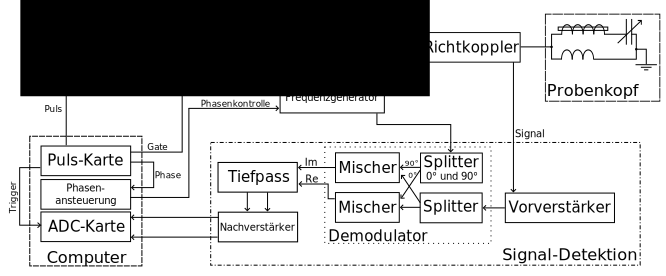
\includegraphics[width=\textwidth]{graphics/joachim/aufbau.pdf} 
	\end{center}
	\caption{Skizzierter Aufbau eines NMR-Spektrometers. Abbildung aus \cite[S. 29]{lueg_implementierung_2016}} \label{fig:exp:aufbau}
\end{figure}

Die Beschreibung nachvollzieht den Aufbau entlang des Signalwegs. Die Steuerung aller Messungen geschieht über einen Computer, der mit der in Python geschriebenen Software DAMARIS (Darmstadt Magnetic Resonance Instrument Software \cite{gadke_damaris_2007}) ausgestattet ist. Diese erlaubt es, Messprogramme zu definieren, mit Hilfe von Pythons serial-Schnittstelle die Verbindung zu verschiedenen Geräten herzustellen, und die produzierten Signale aufzunehmen, anzuzeigen und zur Weiterverarbeitung zu speichern.

Durchgängig läuft ein Frequenzgenerator vom Typ PTS 310, dessen Frequenz auf die Larmorfrequenz des zu untersuchenden Kerns im jeweiligen Magneten eingestellt ist. Ist diese Frequenz nicht bekannt, empfiehlt sich in der Regel das Aufnehmen eines Spektrums von einer Flüssigkeit oder Lösung, die den gewünschten Kern enthält. Aufgrund der geringen Breite des Flüssigkeitsspektrum lässt sich so die magnetfeldabhängige Larmorfrequenz bestimmen.

Soll ein Puls an den Probenkopf gesandt werden, setzt DAMARIS über eine 24-bit-Puls-Karte für die Dauer des Pulses ein Bit auf 1, was mit Hilfe eines HF-Schalters aus dem kontinuierlichen Signal des Frequenzgenerators einen Puls mit der gewünschten Länge ausschneidet.

Dieser Puls wird nun gedämpft. Über diese variable Dämpfung lässt sich die Stärke des Pulses und damit aufgrund der Beziehung $B_\text{Spule} \propto I_\text{Puls}$ das in der Probenspule entstehende Magnetfeld variieren. Dieses wiederum ist nach Formel \eqref{eqn:theo:pulslaenge} entscheidend für die Länge aller Pulse. Es soll die Näherung gelten, dass die während der Pulse stattfindende Dynamik vernachlässigbar ist. Dafür sollte die Dämpfung so eingestellt werden, dass sich die Länge eines Invertierungspulses im Bereich weniger Mikrosekunden befindet.

Der so gedämpfte Puls wird dann mit einem Verstärker der Firma Dressler mit $\SI{2}{\kilo\watt}$ Leistung um einen konstanten Faktor verstärkt und trifft dann über einen Richtkoppler auf den Probenkopf. Der Richtkoppler verhindert dabei, dass der leistungsstarke Puls auf die Detektionselektronik trifft, welche für die Verstärkung \emph{schwacher} Signale ausgelegt ist und entsprechend empfindlich ist.

Das nach dem Puls vom Probenkopf zurückgegebene Signal wird vom Richtkoppler zur Signal-Detektion geleitet. Es wird zunächst von einem Vorverstärker verstärkt, ehe es gesplittet wird. Beide Teile werden mit der vom Frequenzgenerator erzeugten Sinus-Schwingung, welche die Larmorfrequenz hat, gemischt; eine der Schwingungen ist jedoch um $\SI{90}{^\circ}$ phasenverschoben. Die so entstehenden Signale werden Real- und Imaginärteil des Signals genannt. Zusätzlich können beide Teile um eine konstante Phase verschoben werden. Diese lässt sich wiederum über DAMARIS mit einer Phasenansteuerungs-Karte einstellen.

Im nachfolgenden Tiefpass werden alle hochfrequenten Teile des Signals abgeschnitten, sodass nur die durch das Mischen entstandende Differenz $\Delta \omega = \omega_L - \omega_\text{Signal}$ verbleibt. Es lässt sich die Cutoff-Frequenz sowie die Amplitude und der Offset beider Einzelsignale einstellen. Die letzteren Beiden sollten so gewählt sein, dass der Offset Null ist und beide Signale die gleiche Amplitude haben.


Beide Signale werden mit einem Nachverstärker verstärkt, ehe sie von einer ADC-Karte (engl. ADC: Analog-Digital-Konverter) des Computers in Form von Amp\-li\-tu\-den-Wer\-ten in der gesetzten Frequenz von bis zu $\SI{10}{MHz}$ aufgenommen werden. Die ADC-Karte wird dabei über die Puls-Karte mit einem Trigger geschaltet. Dies kann notwendig sein, da vor dem eigentlichen Signal noch unerwünschte Effekte, wie zum Beispiel ein Nachschwingen der Probenspule, auftreten können. Um diese abzuschneiden, kann das Aufnehmen des Signals um eine festgelegte Trigger-Zeit verzögert werden.

Für mehr Informationen zu den hier beschrieben Aufbauten können \cite{lueg_implementierung_2016} und \cite{tilly_master} herangezogen werden.



\section{Weiterverarbeitung der Signale} \label{section:exp:weiterverarbeitung}

Alle so aufgenommen Daten bestehen aus einem Zeitpunkt $t$ und dem zugehörigen Amplitudenwert von Real- und Imaginärteil. Werden Messungen wie eine $T_1$-, $T_2$- oder $F_2$-Messung durchgeführt, ergeben sich variablenabhängige Messreihen. Es wird diese Variable (z.B. Evolutions- oder Mischzeit) meist logarithmisch gegen das Maximum des Realteils der jeweiligen Messung aufgetragen; dann können die Daten analysiert werden. Um ein möglichst großes Realteil-Signal am Ort $t_\text{Max}$ des Maximums zu gewährleisten, sollte dort der Imaginärteil einen Nulldurchgang aufweisen. Dies lässt sich mit einer entsprechenden Einstellung der Phase über die Phasenansteuerungs-Karte erreichen.

Sollen Spektren untersucht werden, wird das Zeitsignal fouriertranformiert. Für eine hohe Auflösung sollte ein möglichst langes Zeitsignal aufgenommen werden; für eine große Spanne ein Zeitsignal mit möglichst hoher Frequenz der ADC-Karte.



\section{Probenköpfe} \label{section:exp:probenkoepfe}

NMR-Messungen bei mehreren Hundert Grad Celsius durchzuführen, kann sich mitunter als eine Herausforderung gestalten. Lötzinne, die häufig verwendet werden um die Resonanzspule an dem Probenkopf anzubringen, schmelzen je nach Art bei weniger als $\SI{200}{\degreeCelsius}$. Aber auch Tuningkondensator und Matchingspule sowie der für die Resonanzspule verwendete Draht sind häufig nur für bestimmte Temperaturen ausgelegt. Zudem ist es offensichtlich, dass für höhere Temperaturen eine gute Isolierung und gegebenenfalls Kühlung des Probenkopfs gegeben sein muss, befindet er doch in direkter Umgebung des mit flüssigem Helium gekühlten Magneten.

Für solche Anwendungen ist also ein spezieller Probenkopf notwendig, welcher in Form des Hochtemperaturprobenkopfs (intern als „Ofen“ bezeichnet) als eine Spezialanfertigung realisiert wurde. Dessen Konstruktionszeichnung ist in Abbildung \ref{fig:exp:ofen_aufbau} zu sehen; eine detaillierte Beschreibung findet sich in \cite{tilly_master}.

\begin{sidewaysfigure}
	\begin{figure}[H]
		\includegraphics[width=1.05\textheight]{graphics/ofen/ofen_aufbau2.pdf}
		\caption{Konstruktionszeichnung des Hochtemperaturprobenkopfes \cite{Rudloff_blue_print}.}
		\label{fig:exp:ofen_aufbau}
	\end{figure}
\end{sidewaysfigure}

Er lässt sich grob in drei Teilen beschreiben: Im oberen Drittel befindet sich der Schwingkreis mit der Probe, eine Vorrichtung, um diese zu erwärmen, sowie die dazugehörige notwendige thermische Isolation. Am unteren Drittel werden alle notwendigen Verbindungen angeschlossen; das mittlere Drittel verbindet beides und beherbergt einen Netzfilter.

Um Temperaturen von bis zu $\SI{1100}{K}$ erreichen zu können, wird ein Heizdraht aus einer FeCrAl-Legierung verwendet. Dieser ist bifilar über einen Hartkeramik-Hohlzylinder gewickelt, um möglichst wenig störende Magnetfelder entstehen zu lassen -- gerade in direkter Umgebung der Probe. Diese Vorrichtung ist im Deckel untergebracht, der sich über die aus Platin bestehende Probenspule stülpen lässt.

Um die entstehende Hitze möglichst gut nach außen hin zu isolieren, ist dieser Aufbau von poröser Keramik umgeben -- sowohl innerhalb des Deckels als auch zwischen Probenspule und Rest des Probenkopfes. Bei letzterem ist zudem eine weitere Scheibe aus dichter Keramik vorhanden. Für die Probenspule und Temperaturfühler sind Bohrungen in den Keramikscheiben vorhanden, über die sie mit dem Rest des Probenkopfes verbunden werden können.

Darunter befindet sich der Schwingkreis der Probenspule. Sowohl eine Matchingspule als auch ein variabler Kondensator und eine Halterung für einen wechselbaren Kondensator sind vorhanden. Es lassen sich Kondensatoren mit verschiedenen Kapazitäten in der Halterung anbringen; zusammen mit dem variablen Kondensator kann so für die Resonanzfrequenz eine Spanne von $\SI{63,6}{MHz}$ bis $\SI{168,9}{MHz}$ (mit Unterbrechungen) abgedeckt werden. Darunter befindet sich die Möglichkeit für eine Wasserkühlung.

Der sich in dem Verbindungsteil befindliche Netzfilter soll den Heizstrom von störenden Anteilen befreien. Dazu wird eine Spule mit eisernem Kern verwendet. Während diese Drossel den Probenkopf in der Vergangenheit genau im Hauptfeld des Magneten gehalten hatte, ist dies jetzt nicht mehr der Fall, was eine hochqualitative Messung sehr schwer macht. Da zudem unerwünschte Einflüsse durch das zusätzliche Magnetfeld zu befürchten sind, liegt die Idee nahe, den vorliegenden Aufbau zu ändern. Eine mögliche Anpassung könnte sein, den Netzfilter außerhalb des Probenkopfes anzubringen und die Positionierung des Probenkopfes im Hauptfeld des Magneten durch eine zusätzliche Halterung zu gewährleisten.

Um den Aufbau zu betreiben, sind im letzten Drittel eine Reihe von Anschlüssen vorhanden:
\begin{itemize}
	\item Ein BNC-Anschluss der vom Richtkoppler kommend zum Schwingkreis führt,
	\item Bohrungen für die beiden Thermoelemente, welche von einem Temperatur-Controller ausgelesen werden,
	\item ein Anschluss für den Heizstrom, welcher von einem Temperatur-Controller bereitgestellt wird,
	\item je eine Rändelstange für die Einstellung von Matching\-spu\-le und Tuningkondensator,
	\item Anschlüsse für Zu- und Abflussschläuche für das Kühlwasser. Der Zufluss kann mit einem Wasserhahn gespeist werden.
\end{itemize}

„Reguläre“ Probenköpfe sind im Vergleich recht einfach gehalten. Da die Temperatursteuerung meist durch den Kryostaten geleistet wird, fallen die Heizeinheit, Isolation, Wasserkühlung und Netzfilter heraus, und es bleiben nur Schwingkreis und Temperaturfühler. In dem hier verwendeten Probenkopf P1 ist zudem keine Matchingspule vorhanden, sodass sich das Abstimmen des Probenkopfs deutlich umständlicher gestaltet und durch eine sehr genaue (und dadurch aufwändigere) Wickelung der Probenspule geleistet werden muss.




\section{Temperaturkontrolle} \label{section:exp:temperaturkontrolle}

Um häufig gewünschte temperaturabhängige Messungen durchführen zu können, lassen sich über Python-Skripte Temperatur-Controller, wie zum Beispiel die hier verwendeten Lakeshore-Einheiten, benutzen. So wird ein Auslesen der aktuellen Temperatur sowie das Setzen einer Soll-Temperatur ermöglicht. Der Temperatur-Controller wiederum steuert Temperatureinheiten im Probenkopf (im Falle des Hochtemperaturprobenkopfs) oder im Kryostaten (im Falle des Probenkopfs P1) an. Die aktuelle Temperatur wird über Temperaturfühler erfasst. Dabei handelt es sich im Falle des Hochtemperaturprobenkopfes um Thermoelemente vom Typ N, im Falle des Probenkopfes P1 um PT100-Elemente ***.





\section{Proben} \label{section:exp:proben}

Bei den durchgeführten Messungen wurden sechs verschiedene Proben verwendet:

\begin{table}[H]
	\centering
	\begin{tabular}{rllllllrl}
		\hline
		ID & Chemikalie & Hersteller & Datum & Glas & Form & \diameter & Foto \\ 
		\hline
		1	& CRN &	C. Zürn &	16.04.97 &	? &	gebogen & 	$\SI{6}{\milli\meter}$ &	(a) \\
2	& CRN &	J. Adam &	13.07.17 &	Duran &	gebogen & 	$\SI{6}{\milli\meter}$ &	(b) \\
3	& CRN &	J. Adam &	30.08.17 &	Duran &	gerade & 	$\SI{5}{\milli\meter}$ &	(c) \\
4	& CRN &	J. Adam &	30.08.17 &	Duran &	gebogen & 	$\SI{5}{\milli\meter}$ &	- *** \\
5	& RbCl in D$_\text{2}$O &	J. Adam &	30.08.17 &	Duran &	gerade & 	$\SI{5}{\milli\meter}$ &	(d) \\
6	& RbCl in D$_\text{2}$O &	J. Adam &	30.08.17 &	Duran &	gebogen & 	$\SI{5}{\milli\meter}$ &	(d) \\ \hline
	\end{tabular} 
	\caption{In dieser Arbeit verwendete Proben. CRN bezeichnet dabei 2Ca(NO$_\text{3}$)$_\text{2}$-3RbNO$_\text{3}$. \label{tab:exp:proben}}
\end{table}

\begin{figure}[H]
	\centering
	\begin{subfigure}{.24\textwidth}
		\centering
		\includegraphics[width=0.95\textwidth]{graphics/proben/CRN_zuern.jpg}
		\caption{ }
		\label{fig:exp:probe_a}
	\end{subfigure}%
	\begin{subfigure}{.24\textwidth}
		\centering
		\includegraphics[width=0.95\textwidth]{graphics/proben/CRN_alt.jpg}
		\caption{ }
		\label{fig:exp:probe_b}
	\end{subfigure}
	\begin{subfigure}{.24\textwidth}
		\centering
		\includegraphics[width=\textwidth]{graphics/proben/CRN_neu.jpg}
		\caption{ }
		\label{fig:exp:probe_c}
	\end{subfigure}
	\begin{subfigure}{.24\textwidth}
		\centering
		\includegraphics[width=\textwidth]{graphics/proben/RbCl_in_D20.jpg}
		\caption{ }
		\label{fig:exp:probe_d}
	\end{subfigure}
	\caption{Fotografien der verwendeten Proben. Die Merkmale finden sich in Tabelle \ref{tab:exp:proben}}
	\label{fig:exp:proben}
\end{figure}

Die Herstellung C. Zürns Probe 1 ist in \cite{zuern_arbeit} dokumentiert.

Die Proben 3 und 4 wurden für diese Arbeit angefertigt. Dafür wurde CRN (was genau für welches? ***) zu einem möglichst feinen Pulver zermörsert und ein gerades bzw. gebogenes Duran-Glas-Röhrchen gefüllt. Um störende Einflüsse von Feuchtigkeit in der Probe möglichst gut zu elimieren, wurden die Proben über Nacht bei $\SI{160}{\degreeCelsius}$ in einem evakuierten Ofen getrocknet, der im Anschluss mit Stickstoffgas gelöscht wurde.

So präpariert wurden die Proben unter Anwendung eines Freeze-Pump-Thaw-Ver\-fah\-rens von Herrn Kollman, Glasbläser der TU Dortmund, abgeschmolzen. Mit dem Verfahren soll der Probe möglichst viel Gas entzogen werden, indem sie Vakuum ausgesetzt wird. Damit die Probe aber nicht mit angesaugt wird, wird sie vor dem Abpumpen eingefroren und danach wieder getaut. Anschließend wurden die Proben durch Erhitzen geschmolzen, um sie dann in einem Glaszustand abkühlen zu lassen.

Mit dem gleichen Verfahren wurde am 13.07.2017 die Probe 2 erstellt, wobei hier die Probe \emph{vor} dem Abschmelzen in den Glaszustand gebracht wurde. Diese Probe wurde jedoch nicht verwendet, da Tests zeigten, dass sie kaum stabil im Glaszustand zu halten war sondern schnell auskristallisierte.

Zum Bestimmen der Larmorfrequenz von $^\text{87}$Rb wurden zudem zwei Proben, Proben 5 und 6, mit in D$_\text{2}$O gelöstem RbCl erstellt. Dabei wurde die gesättigte Lösung in Duran-Glas-Röhrchen eingefüllt und vor dem Abschmelzen möglichst langsam eingefroren, um ein Springen des Röhrchens durch das beim Übergang zum Eis erhöhte Volumen zu verhindern.

\chapter{Experimentelle Resultate und Analysen}
\label{chapter:experiment}

Im Folgenden sollen die im Rahmen dieser Arbeit aufgenommenen Daten vorgestellt und ausgewertet werden. Dabei lassen sich zwei separate Bemühungen unterscheiden. Zum einen wurden Untersuchungen zur Dynamik in CRN angestellt, welche zuerst präsentiert werden sollen, zum anderen wurde die Linienformänderungen in Abhängigkeit der Temperatur untersucht und mit theoretischen Überlegungen verglichen.

Im Verlauf der Auswertung werden die Daten zum Teil nach dem verwendeten Spektrometer unterschieden. Dies liegt an der unterschiedlichen Larmorfrequenzen der Apparaturen -- $\omega_{L, \text{OBI}} = 2\pi \cdot \SI{97.1722}{MHz}$ im Vergleich zu $\omega_{L, \text{Bruker}} = 2\pi \cdot \SI{130.9736}{MHz}$ -- welche sich um etwa einen Faktor $\SI{1.35}{}$ unterscheiden. Dies ist genug, um eine deutliche Auswirkung in den Daten beobachten zu können.

Bei beiden Spektrometern wurden für die grundlegenden Parameter bei allen Messungen etwa die gleichen Einstellungen verwendet: Für das OBI-Spektrometer wurde die Dauer eines $\SI{180}{\degree}$-Pulses auf einen Wert zwischen $\SI{6.5}{\micro s}$ und $\SI{7.1}{\micro s}$ gesetzt, beim Bruker-Spektrometer auf $\SI{5.2}{\micro s}$. Dabei wurde selektiv die Zentrallinie angeregt. Das bedeutet, dass das $^\text{87}$Rb-NMR-Spektrum ist zu breit, als dass es nicht-selektiv angeregt werden könnte, und da es sich bei $^\text{87}$Rb um einen Kern mit halb-zahligen Spin handelt wird nur der Übergang $-\sfrac{1}{2} \leftrightarrow \sfrac{1}{2}$ -- welcher im Spektrum als sogenannte Zentrallinie zu sehen ist -- angeregt.

Die Evolutionszeit $t_p$ der Echos beträgt in den meisten Fällen $\SI{15}{\micro s}$ und nie mehr als $\SI{20}{\micro s}$. Die Wiederholungszeit, also die Zeit zwischen zwei Pulsfolgen, beträgt zwischen $\SI{10}{\milli s}$ und $\SI{50}{\milli s}$. Diese soll dafür sorgen, dass die Magnetisierung nach jeder Pulsfolge wieder in den Ausgangszustand jeder Pulsfolge, der Gleichgewichtsmagnetisierung, zurückkehren kann. Dafür sollte ein Vielfaches der $T_1$-Zeitkonstante gewartet werden.

Der mit dem OBI-Spektrometer abgedeckte Temperaturbereich reicht von $\SI{230}{\kelvin}$ bis $\SI{435}{\kelvin}$, während sich der Temperaturbereich des Bruker-Spektrometers auf den Bereich von $\SI{310}{\kelvin}$ bis $\SI{390}{\kelvin}$ beschränkt.

Alle beschriebenen Fits wurden durch eine least-squares-Methode mit Hilfe von Python-Skripten, welche \texttt{scipy.optimize}- oder \texttt{lmfit}-Routinen verwenden, erstellt.


\section{Bestimmung von $T_1$ und $T_2$} \label{section:res:T_1}

Vor dem Beginn jeder NMR-Messung ist es sinnvoll, $T_1$, die Zeitkonstante der longitudinalen Relaxation, im zu untersuchenden Temperaturgebiet zu vermessen. Dies ist hilfreich, um wichtige Parameter der Messungen abzustecken und mögliche Hindernisse im Vorhinein abschätzen zu können. So sollte zwischen allen Messungen eine Zeit von mindestens $4 T_1$ gewartet werden, um sicherzugehen, dass sich die Magnetisierung in guter Näherung wieder im Gleichgewichtszustand befindet -- wird $T_1$ also im Laufe der Messung bei anderen Temperaturen länger, muss hierauf Rücksicht genommen werden. Wird $T_1$ auf der anderen Seite sehr kurz, kehrt die Magnetisierung sehr schnell in den Gleichgewichtszustand zurück und lassen dem Experimentierenden daher nur ein kleines Fenster, in dem Untersuchungen durchgeführt werden können. Hinzu kommt, dass der Temperaturverlauf von $T_1$ nach Formel \eqref{eqn:bpp} wertvolle Information über die Dynamik in der untersuchten Probe liefern kann. Zuletzt bietet diese recht einfache und reproduzierbare Messung die Möglichkeit, den Aufbau und die Probe auf Übereinstimmung mit Literaturdaten hin zu überprüfen. Daher wurden zu allen untersuchten Temperaturen $T_1$-Messungen aufgenommen.

Zur Bestimmung von $T_1$ wurde eine Invertierungs-Pulsfolge mit Hahn-Echo verwendet.

Repräsentative Rohdaten einer solchen Messung sind in Abbildung \ref{fig:res:T_1_roh} zu sehen. An die Daten wurden Fits mit $T_1$ und $\beta$ als freien Parametern entsprechend Gleichung \eqref{eqn:theo:T_1_fit} angelegt -- diese sind als Linien dargestellt. Die Daten wurden hier zudem auf den Bereich zwischen $1$ und $-1$ normiert, um einen besseren Vergleich zuzulassen. Es ist zu erkennen, dass die Fits eine gute Repräsentation der Daten ermöglichen.
\begin{figure}
	\begin{center}
		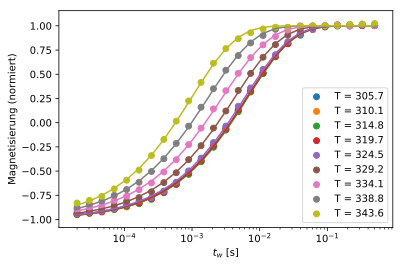
\includegraphics[width=.9\textwidth]{graphics/plot/t1_roh2.pdf}
	\end{center}
	\caption{Aufbaukurven der longitudinalen Magnetisierung zur Bestimmung von $T_1$. Linien stellen Kohlrausch-Fits an die Datenpunkte dar. Die Daten wurden auf $M_{T_1}(0)$ und $M_{T_1}(\infty)$ der Fits normiert.} \label{fig:res:T_1_roh}
\end{figure}

Während sich die Kurven zwischen $\SI{305}{\kelvin}$ und $\SI{325}{\kelvin}$ sehr ähneln, verschieben sich die Kurven und damit auch die $T_1$-Werte bei höheren Temperaturen zu kürzeren Zeiten.

Dies lässt sich auch in der Gesamtübersicht aller aufgenommenen $T_1$-Daten in Abbildung \ref{fig:res:T_1} erkennen. Während die $T_1$-Zeiten bei Temperaturen von $\SI{250}{\kelvin}$ bis $\SI{325}{\kelvin}$ nahezu unverändert im unteren Millisekunden-Bereich liegen, verkürzen sie sich bei steigenden Temperaturen bis in den zweistelligen Mikrosekunden-Bereich. Es ist ein $T_1$-Minimum bei etwa $\SI{390}{\kelvin}$ mit einem Wert von ungefähr $\SI{20}{\micro s}$ auszumachen, ehe die $T_1$-Zeiten stagnieren oder sogar länger werden.
\begin{figure}
	\begin{center}
		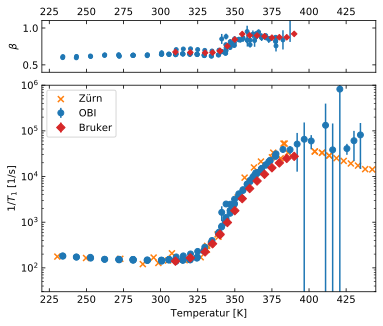
\includegraphics[width=.9\textwidth]{graphics/plot/t1.pdf}
	\end{center}
	\caption{$T_1$ und $\beta$ aus Fits nach Gleichung \eqref{eqn:theo:T_1_fit}. Blaue und rote Symbole zeigen die am OBI- bzw. Bruker-Spektrometer aufgenommen Daten. Bei Temperaturen über $\SI{390}{\kelvin}$ wurden die $\beta$ der Fits auf $\SI{1}{}$ festgesetzt -- diese Werte wurden mit Sternen anstatt Punkten symbolisiert. Orangene Dreiecke bieten einen Vergleich mit Daten von Zürn \cite{zuern_paper}.} \label{fig:res:T_1}
\end{figure}

Während die Unsicherheiten der Fits die Größe der dargestellten Symbole meist nicht überschreiten, sind starke Schwankungen über $\SI{390}{\kelvin}$ zu erkennen. Einem Großteil der dort aufgenommenen Daten kann nicht mehr Bedeutung als einer groben Idee der Tatsachen zugemessen werden.

Abgesehen von dem erwähnten Temperaturbereich ist eine gute Übereinstimmung zu den $T_1$-Daten von Zürn \cite{zuern_paper} und zwischen mehrfach durchgeführten Messungen mit überlappenden Temperaturbereichen zu erkennen, was darauf schließen lässt, dass diese Daten gut reproduzierbar sind. Die am Bruker-Spektrometer aufgenommenen Daten folgen dem gleichen, beschriebenen Verlauf und zeigen bis auf den Temperaturbereich zwischen $\SI{360}{\kelvin}$ und $\SI{390}{\kelvin}$ keinen nennenswerte Differenzen; dort aber sind die gemessenen $T_1$-Daten zu leicht längeren Zeiten verschoben. Der Quotient der $T_1$-Zeiten der beiden Spektrometer überschreitet den Wert $\SI{2}{}$ jedoch nicht.

Im oberen Teil der Abbildung \ref{fig:res:T_1} sind die entsprechenden $\beta$ der Fits zu sehen. Von einem Wert von $\SI{0.6}{}$ bei tieferen Temperaturen steigen sie zu einem Wert von etwa $\SI{0.9}{}$ bei Temperaturen über $\SI{350}{\kelvin}$. Dies entspricht etwa den Ergebnissen von Zürn.

Abweichungen gibt es lediglich bei den höheren Temperaturen, wo $\beta$ laut \cite{zuern_paper} nahe $\SI{1.0}{}$ liegt -- welches hier nicht ganz erreicht wird --, allerdings mit größeren Messunsicherheiten, welche auch hier bei Temperaturen über $\SI{350}{\kelvin}$ zu beobachten sind. Werte über $\SI{390}{\kelvin}$ wurden ausgelassen, da die Messunsicherheiten teils Größenordnungen über dem eigentlichen Wert lagen und somit zu groß waren, als dass den Werten eine Aussage zugestanden werden könnte. Diese Messunsicherheiten stammen daher, dass mit den verwendeten Apparaturen nicht verlässlich Datenpunkte vor $\SI{10}{\micro s}$ aufgenommen werden können. Wenn die $T_1$ Zeit aber in der gleichen Größenordnung liegt und zum Zeitpunkt des $T_1$-Werts das Signal auf etwa $1/e$ abgefallen ist, ist es verständlich, dass ein Fit Schwierigkeiten bereiten kann. Lösen ließe sich dies theoretisch mit einer längeren Evolutionszeit des verwendeten Echos, dies ist aufgrund der kurzen $T_1$- und $T_2$-Zeiten in diesem Temperaturbereich jedoch nicht möglich -- das entstehende Signal ist zu klein um effektiv vom Rauschen getrennt zu werden.

Dennoch ist auffällig, dass trotz der Unsicherheiten von $\beta$ eine relativ gute Übereinstimmung mit den Daten von Zürn vorliegt -- auch von zwei Messreihen zwischen $\SI{315}{\kelvin}$ und $\SI{340}{\kelvin}$ produzierte $\beta$ mit einer Differenz von etwa $\SI{0.1}{}$, sind die zugehörigen $T_1$ in Übereinstimmung miteinander und mit der Literatur. Dies gibt ein Indiz, welche Aussagekraft den exakten Werten von $\beta$ zugemessen werden kann.

Die Unsicherheiten der mit dem Bruker-Spektrometer bestimmten $\beta$ ist vergleichsweise gering. Dies ist mit der höheren Qualität der Daten (besonders auch bei den Linienformen der Spektren in Abbildung \ref{fig:res:bruker_linienform} im Vergleich zu \ref{fig:res:spek_linienform} zu erkennen) und den niedrigeren $T_1$-Werten zu erklären.



% \section{$T_2$} \label{section:res:T_2}
\par\bigskip


Ähnlich wie $T_1$ ist auch $T_2$ eine wichtige Größe, die Parameter für folgende Messungen bestimmen kann -- so werden beispielsweise die praktikablen Längen von Echos von $T_2$ begrenzt. Zudem kann nach Formel \eqref{eqn:theo:T_2_dyn} Aufschluss über Dynamiken gegeben werden.

In Abbildung \ref{fig:res:T_2_roh} sind exemplarisch Rohdaten verschiedener Temperaturen zu sehen. Diese wurden mit einem Hahn-Echo mit $\tau = \SI{15}{\micro s}$ aufgenommen und auf den Bereich zwischen $\SI{0}{}$ und $\SI{1}{}$ normiert.
\begin{figure}
	\begin{center}
		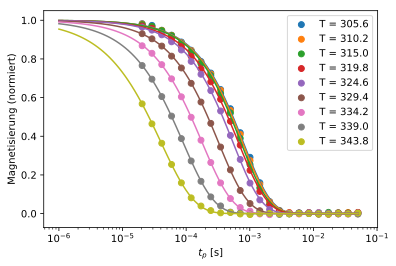
\includegraphics[width=.9\textwidth]{graphics/plot/t2_roh2.pdf}
	\end{center}
	\caption{Kurven des transversalen Magnetisierungszerfalls zur Bestimmung von $T_2$. Linien stellen Kohlrausch-Fits an die Datenpunkte dar. Die Daten wurden auf $M_{T_2}(0)$ und $M_{T_2}(\infty)$ der Fits normiert.} \label{fig:res:T_2_roh}
\end{figure}

An diese wurden Fit-Funktionen nach \eqref{eqn:theo:T_2_fit} angelegt, welche als Linien dargestellt sind. Es lässt sich mit den Fits eine gute Übereinstimmung zu den Daten erzielen. Auch hier lässt sich erkennen, dass $T_2$ bei Temperaturen bis etwa $\SI{320}{\kelvin}$ nahezu konstant verbleibt, und zu hoheren Temperaturen kleiner wird.

Abbildung \label{fig:res:T_2} zeigt eine Übersicht über die aufgenommen $T_2$-Werte mit den zugehörigen $\beta$ der Fits. Unter $\SI{320}{\kelvin}$ verbleiben erstere im niedrigen Millisekunden-Bereich, ehe sie deutlich kürzer werden und sich bei etwa $\SI{360}{\kelvin}$ ein Minimum zeigt. Die Werte des Bruker-Spektrometers sind hiermit in guter Übereinstimmung, wobei wiederum festzuhalten ist, dass die Messunsicherheiten geringer sind. Ein zweites Minimum zeigt sich bei etwa $\SI{400}{\kelvin}$, dessen Wert sich, ebenso wie der erste, im zweistelligen Mikrosekunden-Bereich befindet. Zwischen $\SI{400}{\kelvin}$ und $\SI{410}{\kelvin}$ ist zu erkennen, dass -- wohl durch die Kürze von $T_2$ bei diesen Temperaturen -- deutlich größere Unsicherheiten als im Rest der Messreihe vorliegen, wo sie in guter Näherung vernachlässigbar sind.
\begin{figure}
	\begin{center}
		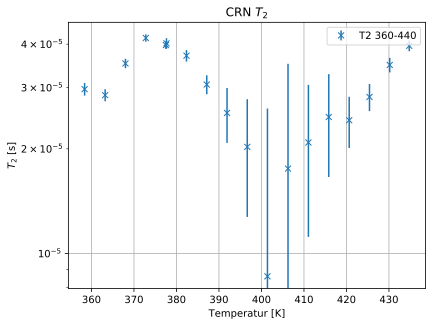
\includegraphics[width=.9\textwidth]{graphics/plot/t2.pdf}
	\end{center}
	\caption{$T_2$ und $\beta$ aus Fits nach Gleichung \eqref{eqn:theo:T_2_fit}. Blaue und rote Symbole zeigen die am OBI- bzw. Bruker-Spektrometer aufgenommen Daten. Bei Temperaturen über $\SI{390}{\kelvin}$ wurden zusätzlich Fits mit einem konstanten $\beta = \SI{1}{}$ erstellt -- diese Werte wurden mit Sternen anstatt Punkten symbolisiert.} \label{fig:res:T_2}
\end{figure}

Auch die $\beta$-Werte zeigen bei höheren Temperaturen deutlich größere Unsicherheiten, hier allerdings schon zwischen $\SI{390}{\kelvin}$ und $\SI{425}{\kelvin}$, was eine Bestimmung der Werte verkompliziert. Sie scheinen zwischen $\SI{1}{}$ und $\SI{2}{}$ zu liegen. Bei tieferen Temperaturen klärt sich das Bild etwas: Während die Daten des OBI-Spektrometers bei Temperaturen bis $\SI{350}{\kelvin}$ ein $\beta$ zwischen $\SI{1}{}$ und $\SI{1.5}{}$ suggerieren, zeigen die Daten des Bruker-Spektrometers ein $\beta$ um $\SI{1}{}$ -- mit geringerer Unsicherheit. Bei nochmals tieferen Temperaturen scheint $\beta$ konsistent bei rund $\SI{1}{}$ zu liegen.




\section{Untersuchung zur Dynamik von CRN} \label{section:res:F_2}

Mit der Absicht einen möglichen Betaprozess zu identifizieren, wurden $F_2$-Messungen und pulslängenabhängige Spektren erstellt; die verwendeten Methoden und Ergebnisse sollen im Folgenden vorgestellt werden

\subsection{Stimulierten Echos} \label{section:res:stimechos}

Es wurden am Spektrometer OBI $F_2$-Messungen, also stimulierte Echos, über eine Reihe von Temperaturen von $\SI{230}{\kelvin}$ bis $\SI{310}{\kelvin}$ und Evolutionszeiten von $\SI{50}{\micro s}$ bis $\SI{1000}{\micro s}$ durchgeführt. Es wurde eine Drei-Puls-Folge verwendet und so sowohl Cos-Cos- als auch Sin-Sin-Korrelation gemessen.

Die meisten Messungen ähnelten der hier beispielhaft ausgewählten bei $\SI{280}{\kelvin}$ und einer Evolutionszeit von $t_p = \SI{1000}{\micro s}$: Die Daten lassen sich schwerlich oder gar nicht von einer $T_1$-Kurve unterscheiden, die bei gleicher Temperatur aufgenommen wurde, wie in Abbildung \ref{fig:res:F_2_tieftemp} oben zu sehen. Es scheint daher nicht möglich, in diesem Temperaturbereich mit dieser Methode Aussagen über mögliche Dynamik treffen zu können.
\begin{figure}
	\centering
	\begin{subfigure}{\textwidth}
		\centering
		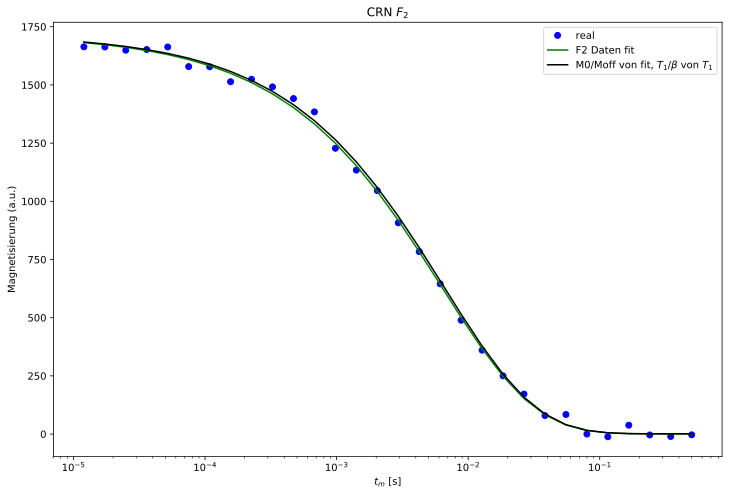
\includegraphics[width=0.9\textwidth]{graphics/plots/F2/f2_tieftemp.pdf}
		% \label{fig:res:F_2_tieftemp}
	\end{subfigure} \\
	\begin{subfigure}{\textwidth}
		\centering
		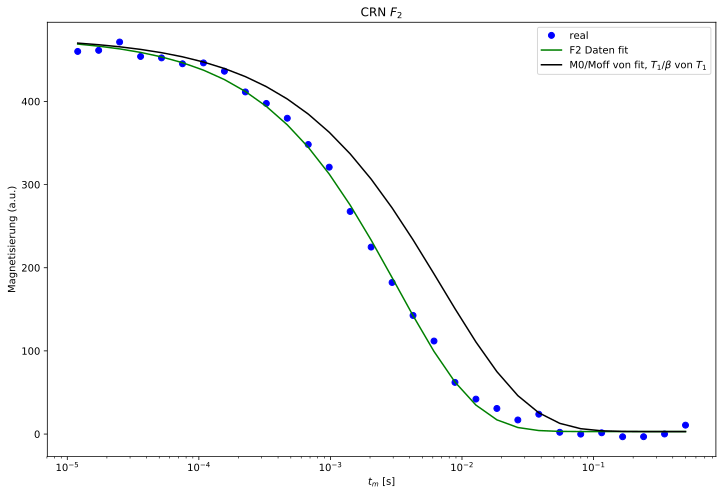
\includegraphics[width=0.9\textwidth]{graphics/plots/F2/f2_fits.pdf}
		% \label{fig:res:F_2_fit}
	\end{subfigure}
	\caption{Oben $F_2$ Messungen bei $\SI{280}{\kelvin}$, unten bei $\SI{310}{\kelvin}$. Grüne Linie zeigt einen Fit an die Daten, schwarze Linie zeigt den Fit mit der Zeitkonstante und $\beta$ ersetzt durch $T_1$ und $\beta_{T_1}$. Bei $\SI{280}{\kelvin}$ sind die Kurven sind fast identisch, was heißt, dass die Kurven keine Dynamik außer $T_1$ zeigen. Bei $\SI{310}{\kelvin}$ ist ein deutlicher Unterschied zwischen den Kurven zu erkennen, was auf stattfindende Dynamik hinweist.}
	\label{fig:res:F_2_tieftemp}
	\label{fig:res:F_2_fit}
\end{figure}

Lediglich bei den Temperaturen $\SI{300}{\kelvin}$ und $\SI{310}{\kelvin}$, sowie $t_p = \SI{1000}{\micro s}$ konnte ein nennenswerter Unterschied zu reinen $T_1$-Kurven beobachtet werden; die entsprechenden Messungen sollen im Folgenden besprochen werden.

Einen Fit der Form *** (Formel stim. Echo) direkt an die Messwerte anzulegen erwies sich als schwierig, daher wurde folgende Schritte für eine Auswertung durchgeführt: An die Daten wurde folgende Funktion gefittet:
\begin{align}
	M_{F_2} (t_m) = M_0 \left[ \exp{ \left(- { \left( \frac{t_m}{\tau_2} \right) }^{\beta_{F_2}} \right)} \right] + M_\text{off} \label{eqn:res:F_2_fit}
\end{align}
Dieser Fit stellt die grüne Kurve in der unteren Hälfte von Abbildung \ref{fig:res:F_2_fit} dar.

Die Werte $\tau_2$ und $\beta_{F_2}$ wurden dann durch $T_1$ und $\beta_{T_1}$ einer $T_1$-Messung gleicher Temperatur ersetzt -- das Resultat ist als schwarze Kurve gezeigt. Dieses Vorgehen macht es möglich, die $T_1$-Kurve an die $F_2$-Daten anzupassen. Es wurden nun die Daten durch die angepasste $T_1$-Kurve geteilt um den entsprechenden Anteil zu eliminieren. Das Resultat ist in Abbildung \ref{fig:res:F_2_T_1} gezeigt.
\begin{figure}
	\begin{center}
		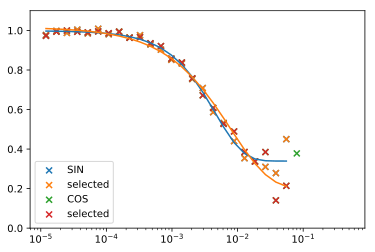
\includegraphics[width=.9\textwidth]{graphics/plots/F2/f2_fit.pdf}
	\end{center}
	\caption{$F_2$-Daten bei $\SI{310}{\kelvin}$ geteilt durch mit $T_1$ und $\beta_{T_1}$ modifiziertem Fit. An die entstandenden Daten wurden Kohlrausch-Fits (dargestellt als Linien) angelegt um Zeitkonstanten zu gewinnen.} \label{fig:res:F_2_T_1}
\end{figure}

Da die Daten bei Mischzeiten von über $\SI{100}{\milli s}$ stark streuen wurden sie nicht dargestellt und aus der Analyse ausgeschlossen, um das Ergebnis nicht zu beeinträchtigen. An verbleibenden Punkte wiederum kann ein Kohlrausch-Fit angelegt werden, um über den beschriebenen Umweg zu einer Funktion ähnlich der aus Formel (*** stim. Echo) zu gelangen.

Es wurden je zwei Messungen einer Cos-Cos-Pulsfolge und einer Sin-Sin-Pulsfolge bei $\SI{310}{\kelvin}$ durchgeführt, sowie je eine Messung bei $\SI{300}{\kelvin}$. Die Resultate finden sich in Tabelle \ref{tab:res:F_2} und später in Abbildung \ref{fig:res:dynvgl}.
\begin{table}
	\centering
	\begin{tabular}{lllll}
		\hline
		Temperatur & Sin-Sin $\tau$ & Sin-Sin $\beta$ & Cos-Cos $\tau$ & Cos-Cos $\beta$ \\ \hline
		$\SI{300}{\kelvin}$ (Lauf 1) & $\SI{5.26 (94)}{\milli s}$ & $\SI{0.95 (18)}{}$ & $\SI{3.68 (63)}{\milli s}$ & $\SI{1.30 (34)}{}$ \\
		$\SI{310}{\kelvin}$ (Lauf 1) & $\SI{3.27 (122)}{\milli s}$ & $\SI{1.12 (56)}{}$ & $\SI{9.95 (432)}{\milli s}$ & $\SI{0.74 (21)}{}$ \\
		$\SI{310}{\kelvin}$ (Lauf 2) & $\SI{4.23 (37)}{\milli s}$ & $\SI{1.01 (10)}{}$ & $\SI{3.28 (7)}{\milli s}$ & $\SI{0.71 (1)}{}$ \\
		 \hline
	\end{tabular}
	\caption{Resultate der $F_2$-Messungen. Sin-Sin und Cos-Cos beziehen sich auf die jeweils verwendete Pulsfolge, $\tau$ und $\beta$ sind die mit den Fits bestimmten Parameter der Zeitkonstante und der Streckung der Exponentialfunktion. \label{tab:res:F_2}}
\end{table}

Es ist zu erkennen, dass die Größen zwischen den zwei Durchläufen teils mehr schwanken als zwischen zwei Temperaturen oder im Vergleich zwischen Sin-Sin- und Cos-Cos-Pulsfolgen. Da die Unsicherheiten zudem in Fällen beinahe $\SI{50}{\percent}$ erreicht, müssen diese Ergebnisse mit Vorsicht betrachtet werden.



\subsection{Pulslängenabhängige Spektren} \label{section:res:spekdyn}

Eine weitere Untersuchung zu möglicher Dynamik wurde an der sich ändernden Linienform von pulslängenabhängigen Spektren durchgeführt. Während hier nur auf die Bestimmung von Zeitkonstanten eingegangen werden soll, werden die Details von CRN-Spektren im späteren Abschnitt \ref{section:res:spektren} diskutiert.

Es wurde beobachtet, dass Spektren, die mit einem Hahn-Echo mit unterschiedlicher Evolutionszeit aufgenommen wurden, eine unterschiedliche Linienform zeigen. Die Halbwertsbreiten der normierten Spektren sind also evolutionszeitabhängig, und das bei verschiedenen Temperaturen in verschiedenen Maßen. Dies lässt sich in Abbildung \ref{fig:res:spekdyn_305K} im Vergleich mit Abbildung \ref{fig:res:spekdyn_325K} erkennen, wo pulslängenabhängige Spektren für die Temperaturen $\SI{305}{\kelvin}$ bzw. $\SI{325}{\kelvin}$ gezeigt sind.
\begin{figure}
	\begin{center}
		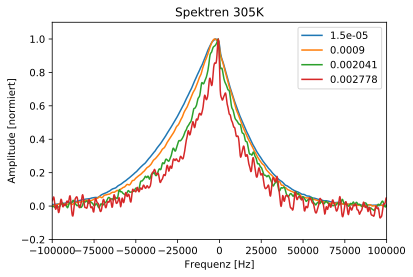
\includegraphics[width=.8\textwidth]{graphics/plots/SPEKDYN/spekdyn_305K.pdf}
	\end{center}
	\caption{Änderung der Linienform der Spektren bei $\SI{305}{\kelvin}$ in Abhängigkeit der Evolutionszeit $t_p$.} \label{fig:res:spekdyn_305K}
\end{figure}
\begin{figure}
	\begin{center}
		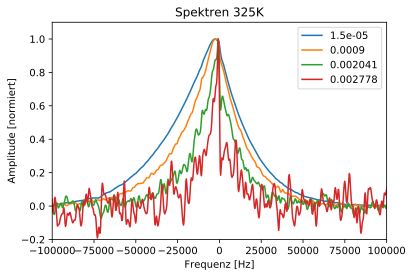
\includegraphics[width=.8\textwidth]{graphics/plots/SPEKDYN/spekdyn_325K.pdf}
	\end{center}
	\caption{Änderung der Linienform der Spektren bei $\SI{325}{\kelvin}$ in Abhängigkeit der Evolutionszeit $t_p$. Im Vergleich zu \ref{fig:res:spekdyn_305K} ist eine deutlich stärkere Verschmälerung zu hohen $t_p$ zu erkennen.} \label{fig:res:spekdyn_325K}
\end{figure}
Alle Spektren wurden mit dem OBI-Spektrometer aufgenommen; dabei wurde ein Hahn-Echo mit variabler Evolutionszeit verwendet und die Spektren mit $\SI{500}{Hz}$ apodisiert.

Zur Untersuchung dieses Phänomens wurde für jede Temperatur die Halbwertsbreite gegen die Evolutionszeit $t_p$ aufgetragen. Da die Spektren bei hohen Pulslängen teils sehr verrauscht sind, wurden die verwendeten Evolutionszeiten auf $\SI{2}{\milli s}$ begrenzt um Fits nicht ungünstig zu beeinflussen. An diese Daten wurden Kohlrausch-Fits angelegt, die als durchgezogene Linien, zusammen mit dem Daten, in Abbildung \ref{fig:res:spekdyn_fits} zu sehen sind.
\begin{figure}
	\begin{center}
		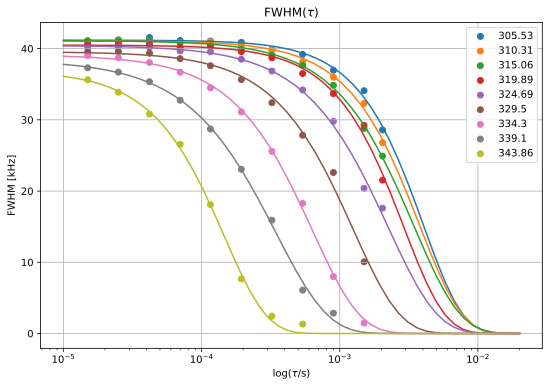
\includegraphics[width=.9\textwidth]{graphics/plots/SPEKDYN/spekdyn_fits.pdf}
	\end{center}
	\caption{Halbwertsbreiten in Abhängigkeit von $t_p$. An diese Daten wurden Kohlrausch-Fits angelegt, dargestellt als durchgezogene Linien.} \label{fig:res:spekdyn_fits}
\end{figure}

Es wurde eine weitere, ähnliche Auswertung wurde durchgeführt, wobei anstatt der Halbwertsbreite die Amplitude bei einer bestimmten Frequenz (beispielsweise bei $\SI{-15}{\kilo Hz}$) als Variable genommen wurde. Die Ergebnisse glichen der der Halbwertsbreiten-Betrachtung, waren aber durchgehend mit größeren Unsicherheiten behaftet. Dies lässt sich durch die stark verrauschten Spektren bei hohen Evolutionszeiten erklären, die zu stark schwankenden Amplituden führen, welche wiederum einen guten Fit der Daten schwierig gestalten.



\subsection{Auswertung der experimentell bestimmten Zeitkonstanten} \label{section:res:dynausw}

Werden die bestimmten Zeitkonstanten der $T_1$-, $T_2$-, $F_2$- und $t_p$-abhängigen Spektrums-Messungen zusammen mit dem Fit der Werte des $\beta$-Prozesses (vlg. Abbildung ***) aufgetragen, ergibt sich das in Abbildung \ref{fig:res:dynvgl} gezeigt Bild.
\begin{figure}
	\begin{center}
		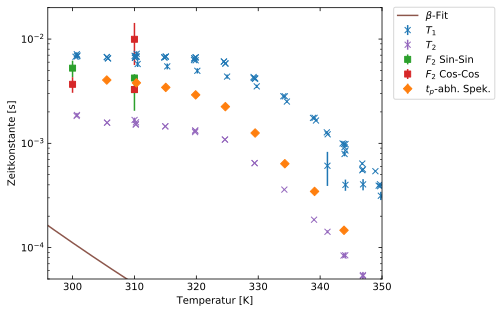
\includegraphics[width=.9\textwidth]{graphics/plot/dyn.pdf}
	\end{center}
	\caption{Vergleich der gewonnenen Zeitkonstanten.} \label{fig:res:dynvgl}
\end{figure}
Alle bestimmten Zeitkonstanten liegen -- im Rahmen der Unsicherheiten -- zwischen den bestimmten $T_1$- und $T_2$-Werten. Diese Unsicherheiten sind bei fast allen Messungen, mit Ausnahme der $F_2$-Messungen, unter der verwendeten Symbolgröße und können vernachlässigt werden. Die höheren Unsicherheiten der $F_2$-Messungen sind ob der verwendeten, mehrschrittigen Auswertung verständlich.

Ab $\SI{320}{\kelvin}$ bis $\SI{330}{\kelvin}$ zeigen alle Zeitkonstanten einen Übergang zu kürzeren Zeiten, der wohl mit der höheren Bewegung der Atome in der Nähe der Glasübergangstemperatur von $T_g = \SI{333}{\kelvin}$ einhergeht. Dieser Effekt ist auch als Bewegungsverschmälerung in Spektren zu sehen (vgl. Abbildung \ref{fig:res:spek_fwhm}).

Die braune Linie stellt dabei einen Fit durch die in Abbildung (*** Bild Zürn Paper) gezeigten, zum $\beta$-Prozess gehörenden Werte dar, um eine Abschätzung zu geben, in welcher Größenordnung der Prozess im untersuchten Temperaturbereich liegt, sollte sich der angedeutete Trend linear fortsetzen. Wie zu erkennen, befindet sich keine der bestimmten Zeitkonstanten in der entsprechenden Größenordnung. Dies bedeutet entweder, dass der Prozess mit den verwendeten Methoden nicht detektiert werden konnte -- möglicherweise aufgrund eines zu geringen Einflusses --, oder, dass die Grundannahme eines $\beta$-Prozesses in dieser Größenordnung in diesem Temperaturbereich in CRN nicht korrekt ist. Weitere Untersuchungen sind nötig, um diese Frage abschließend klären zu können.



\section{Linienform von experimentellen und simulierten CRN-Spektren} \label{section:res:spektren}

Das zweite Ziel dieser Arbeit ist die Untersuchung der Linienform von CRN-Spektren. Bei der Auswertung von Spektren wurde eine zunächst ungewöhnlich erscheinende Verbreiterung derselben in einem Temperaturbereich beobachtet, wo, aufgrund von Bewegungsverschmälerung, eher kleinere Halbwertsbreiten zu erwarten wären. Zur Untersuchung der Gegebenheiten wurden, neben einer Vielzahl von experimenteller Spektren, Computer-Simulationen angefertigt, und versucht eine theoretische Erklärung der Daten zu bieten.

\begin{figure}
	\begin{center}
		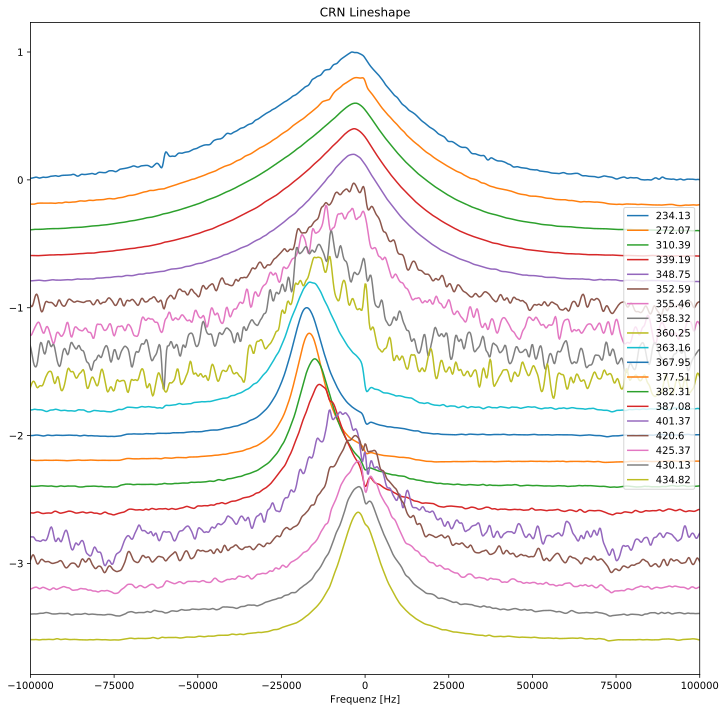
\includegraphics[width=\textwidth]{graphics/plot/spek_lineshape.pdf}
	\end{center}
	\caption{Vergleich der Linienform von am OBI-Spektrometer aufgenommen Spektren.} \label{fig:res:spek_linienform}
\end{figure}
Um eine Übersicht zu schaffen, werden zuerst die Linienformen der Spektren aus den verschiedenen Quellen in Abhängigkeit der Temperatur präsentiert. Abbildung \ref{fig:res:spek_linienform} zeigt die am OBI-Spektrometer aufgenommenen Spektren; die Temperaturen reichen von etwa $\SI{234}{\kelvin}$ bis etwa $\SI{435}{\kelvin}$. Sie wurden mit einem Hahn-Echo mit einer Evolutionszeit von $t_p = \SI{15}{\micro s}$ aufgenommen und mit $\SI{500}{Hz}$ apodisiert. Es wurden je $\SI{8192}{}$ Datenpunkte mit einer Frequenz von $\SI{2}{MHz}$ erstellt. Die Spektren wurden in mehreren Messreihen aufgenommen und stellen eine repräsentative Auswahl dar, die es erlaubt, den Verlauf der Linienform nachzuvollziehen, ohne zu stark an Übersicht zu verlieren.

Bei tiefen Temperaturen ist eine Form zu beobachten, die der des Czjzek-Spektrums aus Kapitel (***) ähnelt. Diese hält sich über weite Temperaturen, von etwa $\SI{235}{\kelvin}$ bis etwa $\SI{350}{\kelvin}$, fast unverändert. Zu höheren Temperaturen ändert sich die Linienform, sie nimmt die einer Lorentz-Funktion
\begin{align}
	L(f) = \frac{1}{\pi \gamma} \cdot \frac{\gamma^2}{\gamma^2 + (f - f_0)^2} \label{eqn:res:lorentz}
\end{align}
an, während die Spektren gleichzeitig schmaler werden und sich der Schwerpunkt zu niedrigeren Frequenzen verschiebt. Diese Bewegung findet ein Ende bei etwa $\SI{367}{\kelvin}$: Zu höheren Temperaturen verbreitern sich die Spektren wieder, ehe sie ab $\SI{410}{\kelvin}$ wieder schmaler werden. Der Schwerpunkt verschiebt sich ab 375K wieder gegen $\SI{0}{Hz}$, wo es ab 400K verweilt. Die Linienform ändert sich nicht mehr.

Es ist auffällig, dass die Qualität der Spektren stark mit der Temperatur schwankt. Zwischen $\SI{235}{\kelvin}$ und $\SI{350}{\kelvin}$, $\SI{363}{\kelvin}$ und $\SI{387}{\kelvin}$, sowie zwischen $\SI{430}{\kelvin}$ und $\SI{435}{\kelvin}$ weisen die Spektren vergleichsweise geringes Rauschen und somit eine glattere Form auf. Die abschnittweise höheren Schwankungen lassen sich durch $T_2$-Minima (siehe Abbildung \ref{fig:res:T_2}) bei den entsprechenden Temperaturen erklären -- diese sorgen für einen schnellen Abfall des Signals und entsprechend verrauschte Spektren.

\begin{figure}
	\begin{center}
		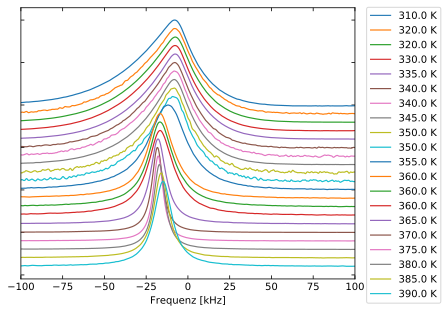
\includegraphics[width=\textwidth]{graphics/plot/bruker_lineshape.pdf}
	\end{center}
	\caption{Vergleich der Linienform von am Bruker-Spektrometer aufgenommen Spektren.} \label{fig:res:bruker_linienform}
\end{figure}
Die am Bruker-Spektrometer aufgenommenen Spektren decken einen Temperaturbereich von $\SI{310}{\kelvin}$ bis $\SI{390}{\kelvin}$ ab, und wurden ebenfalls mit einem Hahn-Echo mit einer Evolutionszeit von $\SI{15}{\micro s}$ erstellt und mit $\SI{500}{Hz}$ apodisiert. Hier wurden je $\SI{4096}{}$ Datenpunkte mit einer Frequenz von $\SI{0.5}{MHz}$ aufgenommen. Da mit diesem Spektrometer weitaus weniger Spektren erstellt wurden als mit dem OBI-Spektrometer können in Abbildung \ref{fig:res:bruker_linienform} alle erstellten Spektren präsentiert werden.

Der Verlauf der Linienform gleicht der beschriebenen in dem entsprechenden Temperaturbereich gut. Es ist das geringe Rauschen der Spektren zu beachten, das, wie auch insbesondere die $T_2$-Daten, ein Beleg für hohe Datenqualität des Bruker-Spektrometers in diesem Kontext ist.

Als Ergänzung zu den experimentellen Daten wurden Spektren simuliert. Dazu wurde die in Kapitel (***) vorgestellte Simulations-Software verwendet. Es wurden FIDs mit $\SI{4096}{}$ Datenpunkten mit einem Abstand von je $\SI{0.5}{\micro s}$, was einer Frequenz von $\SI{2}{MHz}$ entspricht, aufgenommen. Um einen Mittelwert zu bilden wurden, je nach Spektrum, zwischen $10^{7}$ und $10^{9}$ einzelne Trajektorien gemittelt. Als Modell wurde ein isotroper Zufallssprung gewählt, welcher eine Czjzek-Verteilung als Ausgangspunkt hat; dieses war der simulierten Quadrupol-Wechselwirkung zweiter Ordnung ausgesetzt. Zur Bestimmung der Lebensdauer eines bestimmten Zustandes wurde eine Exponentialverteilung genutzt, deren Parameter, die Lebenszeit, eine Verknüpfung mit Temperaturen ermöglicht. Es wurde eine Vogel-Fulcher-Funktion für die Lebenszeit mit den Parametern für CRN aus \cite{PIMENOV199793} verwendet. Zur besseren Vergleichbarkeit werden im Folgenden die Spektren mit den so berechneten Temperaturen anstatt mit den Lebenszeiten referenziert. Die resultierenden Spektren sind in Abbildung \ref{fig:res:sim_linienform} zu sehen. Da die Breite der Spektren in der Simulation mit nur einem frei wählbaren Parameter bestimmt wird, wurde sie durch das Vergleichen der Form bei tiefen Temperaturen normiert.
\begin{figure}
	\begin{center}
		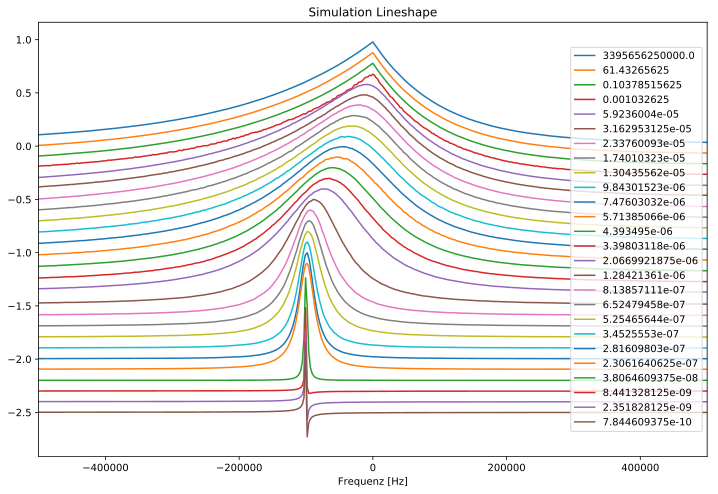
\includegraphics[width=\textwidth]{graphics/plot/sim_lineshape.pdf}
	\end{center}
	\caption{Vergleich der Linienform von mit Simulationen erstellte Spektren. Die angegebenen Temperaturen wurden mithilfe von den in Kapitel \ref{section:res:theorie} beschriebenen $\tau_c$ aus den verwendeten $\tau$ bestimmt.} \label{fig:res:sim_linienform}
\end{figure}

Bei tiefen Temperaturen gleichen die simulierten Spektren den experimentellen; dies wurde schon in \cite{joachim_master} gefunden. Auch ist der Übergang zur Lorentz-Form, verbunden mit der Verschiebung des Schwerpunkts und Verschmälerung der Spektren bei etwa der gleichen Temperatur von $\SI{350}{\kelvin}$ zu beobachten. Im Gegensatz zu den experimentellen Spektren werden die simulierten Spektren mit steigender Temperatur jedoch immer schmaler und ändern den Schwerpunkt nicht mehr.


Um eine quantitative Behandlung der Spektren zu ermöglichen wurden zwei Messgrößen verwendet: Die Halbwertsbreite (also die Breite auf der Höhe der Hälfte des Maximums) und der Schwerpunkt der Spektren. Um bei den stark verrauschten Spektren des OBI-Spektrometers zwischen $\SI{350}{\kelvin}$ und $\SI{360}{\kelvin}$, und zwischen $\SI{390}{\kelvin}$ und $\SI{430}{\kelvin}$ gut vergleichbare Werte zu erhalten, wurde ein Lorentz-Fit nach Gleichung \eqref{eqn:res:lorentz} mit einer least-squares-Methode an die Spektren angelegt. So entspricht $2 \gamma$ der Halbwertsbreite und das Maximum $f_0$, aufgrund der Symmetrie der Funktion, dem Schwerpunkt. Die so gewonnenen Halbwertsbreiten sind in Abbildung \ref{fig:res:spek_fwhm} zu sehen.
\begin{figure}
	\begin{center}
		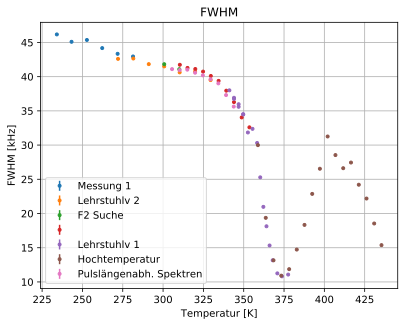
\includegraphics[width=.9\textwidth]{graphics/plot/fwhm.pdf}
	\end{center}
	\caption{Die Halbwertsbreite der Spektren. Blaue und rote Symbole kennzeichnen am OBI- bzw. Bruker-Spektrometer aufgenommene Spektren, grüne Symbole stammen von simulierten Spektren. Der auffälligste Unterschied zwischen experimentellen und simulierten Spektren ist das zusätzliche Maximum bei hohen Temperaturen bzw. das Fehlen dessen.} \label{fig:res:spek_fwhm}
\end{figure}

Es ist zu erkennen, dass die Werte der Halbwertsbreite etwa dem entsprechen, was nach einer Betrachtung der Spektren zu erwarten wäre: Von einem Spektrum mit etwa $\SI{40}{kHz}$ Breite bei niedrigen Temperaturen gehen die Werte zu einem Minimum von etwa $\SI{10}{kHz}$ bei etwa $\SI{375}{\kelvin}$ über, um nach einem lokalen Maximum von rund $\SI{20}{kHz}$ bei etwa $\SI{400}{\kelvin}$ erneut abzufallen.

Diesem Verlauf der am OBI-Spektrometer aufgenommenen Spektren folgen auch die Halbwertsbreiten der am Bruker-Spektrometer produzierten Daten. Letztere liegen allerdings konstant bei niedrigeren Werten. Das Verhältnis entspricht aber auch nicht durchgehend dem Verhältnis $4:3$, was die entsprechend unterschiedlichen Larmorfrequenzen suggerieren würden; es liegt bei tiefen Temperaturen etwas niedriger und bei höheren Temperaturen etwas höher. So ist im Bereich zwischen $\SI{310}{\kelvin}$ und $\SI{350}{\kelvin}$ ein Verhältnis von etwa $\SI{1.15}{}:1$ zu finden, zwischen $\SI{360}{\kelvin}$ und $\SI{390}{\kelvin}$ ein Verhältnis von $\SI{1.45}{}:1$ bis $\SI{1.55}{}:1$. Messungen an einem $\SI{600}{MHz}$-Spektrometer wären hilfreich, um fundiertere Aussagen über Larmorfrequenz-abhängige Effekte treffen zu können.

Der Verlauf der Halbwertsbreiten der simulierten Spektren unterscheidet sich deutlich von dem der experimentellen Spektren. Während der grobe Verlauf übereinstimmt -- von breiten Spektren bei tiefen Temperaturen zu schmalen Spektren bei höheren Temperaturen -- sind bei genauerer Betrachtung starke Abweichungen zu sehen. Die simulierten Spektren werden zu höheren Temperaturen zunehmend schmaler und näheren sich einem Delta-Peak, während die Breiten der experimentellen Spektren ein weiteres Maximum aufweisen. Zudem ist ein Maximum der Halbwertsbreite der simulierten Spektren bei etwa $\SI{345}{\kelvin}$ zu beobachten, während die Halbwertsbreite der experimentellen Spektren einen fließenden Übergang der Breite von hohen zu tiefen Temperaturen zeigen.

Es sollte darauf aufmerksam gemacht werden, dass die Halbwertsbreite stark von der Form der Spitze beeinflusst wird, welche das Maximum und damit die Hälfte des Maximums bestimmt. Sind, wie bei den simulierten Spektren, extrem gut definierte Maxima zu sehen, drückt dies den Wert der Halbwertsbreiten im Vergleich zu den experimentellen Halbwertsbreiten nach unten. Dies erklärt den Abfall der Halbwertsbreiten der simulierten Spektren zu tieferen Temperaturen: Hier sind die scharfe Spitzen der Czjzek-Spektren gut ausgeprägt, sodass die Halbwertsbreite der Spektren beim Übergang zur abgerundeten Lorentz-Form ein Maximum durchläuft. Die experimentellen Spektren hingegen zeigen aufgrund von experimentellen Beschränkungen wie der Auflösung, und möglicherweise durch weitere Effekte, bei niedrigeren Temperaturen keine perfekte Spitze und daher auch keinen Peak in der Halbwertsbreite beim Übergang zur Lorentz-Form.

\par\bigskip

In Abbildung \ref{fig:res:spek_mean} sind die Schwerpunkte der Spektren aufgetragen. Diese wurden mit Hilfe von numerischer Integration nach der Simpsonregel bestimmt. Bei stark verrauschten Spektren, wo dieses Vorgehen wenig Erfolg verspricht -- es wird eher der Schwerpunkt der Schwankungen bestimmt als der des Signals --, wurden wieder Lorentz-Fits ausgenutzt, deren Parameter $f_0$ der Schwerpunkt ist.
\begin{figure}
	\begin{center}
		\includegraphics[width=.9\textwidth]{graphics/plot/mean.pdf} 
	\end{center}
	\caption{Die Halbwertsbreite der Spektren. Blaue und rote Symbole kennzeichnen am OBI- bzw. Bruker-Spektrometer aufgenommene Spektren, grüne Symbole stammen von simulierten Spektren. Während der Schwerpunkt der experimentellen Spektren zu hohen Temperaturen gegen $\SI{0}{\kilo Hz}$ geht, verbleibt der Schwerpunkt der simulierten Spektren bei etwa $\SI{-16}{\kilo Hz}$.} \label{fig:res:spek_mean}
\end{figure}

Allen drei Kurvenverläufe ist gleich, dass sie bei tieferen Temperaturen bis etwa $\SI{360}{\kelvin}$ einen konstanten Wert zeigen, ehe sich der Schwerpunkt zu niedrigeren Frequenzen von etwa $\SI{-16}{\kilo Hz}$ verschiebt, was mit dem Übergang von der Czjzek-Form des Spektrums zur Lorentz-Form einhergeht. Die spezifischen konstanten Werte der tieferen Temperaturen unterscheiden sich jedoch zwischen den Daten des OBI-Spektrometers mit einem Schwerpunkt von etwa $\SI{-8}{\kilo Hz}$, und den Daten des Bruker-Spektrometers und der Simulation mit einem Schwerpunkt von etwa $\SI{-12}{\kilo Hz}$. Auch in diesem Kontext könnten Messungen am Spektrometern mit unterschiedlichen Larmorfrequenz helfen, um beispielsweise den Einfluss der chemischen Verschiebung auf die Position der Schwerpunkte zu untersuchen.

Ab etwa $\SI{375}{\kelvin}$ ist eine Bewegung des Schwerpunkts der experimentellen Spektren zum Nullpunkt zu erkennen, die die Spektren des OBI-Spektrometers aufgrund des größeren abgedeckten Temperaturbereichs auch erreichen. Die simulierten Spektren verbleiben jedoch bei dem Wert von $\SI{-16}{\kilo Hz}$, der bei $\SI{370}{\kelvin}$ erreicht wird.

Auch hier ist einschränkend zu sagen, dass die Werte der Schwerpunkte aufgrund von externen Faktoren instabil sind, mehr noch als die Halbwertsbreiten. Wie in Kapitel \ref{section:exp:weiterverarbeitung} erwähnt, wird eine Phasenanpassung des Real- und Imaginärteils durchgeführt, um ein maximales Signal zu garantieren und mögliche Schwankungen der Phase durch experimentelle Einflüsse auszugleichen. Allerding kann eine Abweichung von $\pm \SI{1}{\degree}$ vom Optimalwert unter den schlechtesten Umständen eine Verschiebung des Schwerpunkts um $\SI{1}{\kilo Hz}$ bewirken. Diese Empfindlichkeit gegenüber kleinen Änderungen bedeutet, dass Schwankungen der dargestellten Werte nicht auszuschließen ist; die groben Merkmale der Kurvenverläufe können aber leicht durch eine Betrachtung der Spektren bestätigt werden.




\section{Vergleich von CRN-Spektren mit theoretischen Überlegungen} \label{section:res:theorie}

Die experimentellen Ergebnisse sollen mit den theoretischen Überlegungen vergleichen werden. Dazu wurden die in Kapitel \ref{section:theo:qww} beschriebenen Funktionen für $T_1$, Halbwertsbreite und Schwerpunkt verwendet. Um eine Übereinstimmung zur Theorie feststellen zu können, müssen sich alle Datensätze mit dem gleichen Satz geteilter Parameter beschreiben lassen. Im Falle der Spektraldichte $J_\text{BPP}$ ist dies $C_Q$; für $J_\text{CC}$ und $J_\text{CD}$ sind $\alpha$ bzw. $\gamma$ zusätzliche Parameter.

Für den Parameter $\eta$ der Spektraldichten wurde $\eta^2 = 42 - 24 \sqrt{3} \approx \SI{0.43}{}$ \cite{caer} verwendet. Nach \cite{PIMENOV199793} wird für CRN für die Korrelationszeit $\tau_c$ ein Vogel-Fulcher-Gesetz
\begin{align}
	\tau_c = \tau_{co} \exp \left( \frac{D T_\text{VF}}{T-T_\text{VF}} \right)
\end{align}
mit dem strength index $D = \SI{3.5}{}$, der Vogel-Fulcher-Temperatur $T_\text{VF} = \SI{294}{K}$ und dem Frequenzfaktor $\tau_{co} = \SI{5.1e-14}{s}$ angenommen. Diese Werte wurden durch dielektrische Spektroskopie gewonnen.

Am $T_1$-Minimum nach Gleichung \eqref{eqn:bpp} gilt $\omega \tau_c \approx \SI{0.61}{}$ \cite[S. 629]{omegatau061}. Das $T_1$-Minimum kann in den OBI-Daten bei etwa $T_{T_1 \text{min}} = \SI{410}{K}$ gefunden werden; die Larmorfrequenz liegt bei $\omega_L = 2\pi \cdot \SI{97.1722}{MHz}$, was bedeutet, dass bei $T_{T_1 \text{min}}$ gilt $\tau_c \approx \sfrac{\SI{0.61}{}}{\omega_L} \approx \SI{1.0}{\nano s}$. Vergleicht man das Vogel-Fulcher-Gesetz mit diesem Punkt, lässt sich erkennen, dass eine gute Übereinstimmung vorliegt.

\begin{wrapfigure}{r}{0.5\textwidth}
	\vspace{-20pt}
	\begin{center}
		\includegraphics[width=0.49\textwidth]{graphics/plot/vftau.pdf}
	\end{center}
	\vspace{-20pt}
	\caption{Vergleich von Zeitkonstante aus $T_1$-Minimum, und Vogel-Fulcher-Gesetz für CRN mit Parametern nach \cite{PIMENOV199793} in orange und Parametern nach \cite{crn_augsburg} in grün. \label{fig:korrelationszeiten}}
\end{wrapfigure}
Ein Vergleich mit den Parametern $D = \SI{4.72}{}$, $T_\text{VF} = \SI{285}{K}$ und $\tau_{co} = \SI{1.15e-14}{s}$ nach \cite{crn_augsburg}, ebenfalls bestimmt durch dielektrische Spektroskopie, ist in den Abbildungen \ref{fig:korrelationszeiten} und \ref{fig:res:theorie_j} zu sehen. Während leichte Unterschiede zu erkennen sind, ändert sich das Gesamtbild wenig, weswegen sich diese Ausführungen auf den ersten Parametersatz beschränken.




Führt man zunächst einen Vergleich der Halbwertsbreiten mit der Theorie durch, lässt sich leicht feststellen, dass signifikante Unterschiede zu beobachten sind: Die gemessenen Halbwertsbreiten sind ab $\SI{360}{\kelvin}$ aufwärts deutlich größer als vorhergesagt. Dies liegt am Einfluss des kurzen $T_1$ von etwa $\SI{50}{\micro s}$, welches mit der zusätzlich Relaxation zur Verbreiterung des Spektrums beiträgt.

Um einen Vergleich mit der Theorie dennoch durchführen zu können, wurde versucht den Einfluss von $T_1$ rechnerisch zu eliminieren. Im Bereich des Einflusses lassen sich die Spektren gut mit einem Lorentz-Fit (vgl. Gleichung \eqref{eqn:res:lorentz}) näheren. Die Fouriertransformierte hiervon ist eine gedämpfte Schwingung mit der Halbwertsbreite $2 \gamma_0 = a/\pi$:
\begin{align}
	h(t) & = \exp{(-a |t|)} \cos{(2 \pi f_0 t)} \\
	H(t) & = \int_{-\infty}^{\infty} h(t) \exp{i 2 \pi f t} \text{d} t \\
	H(f) & = \frac{2}{a} \cdot \frac{(a/2\pi)^2}{((a/2\pi)^2) + (f - f_0)^2}
\end{align}

Diese gedämpfte Schwingung soll durch eine normierte Kohlrausch-Funktion
\begin{align}
	f(t) = \exp{\left( {\left(-\frac{t}{T_1} \right)}^\beta \right) },
\end{align}
welche für Fits an $T_1$ verwendet werden kann, geteilt werden. Da die Messung der Signale per Definition immer bei 0 beginnt, kann $t$ durch $|t|$ ersetzt werden. Für eine vereinfachte Rechnung wird hier wird $\beta = 1$ angenommen, was in der Regel eine annehmbare Näherung darstellt.
\begin{align}
	h'(t) &= \exp{(-a \lvert t \rvert)} \cdot \cos{(2 \pi f_0 t)} \cdot \exp{\left(\frac{|t|}{T_1} \right)} \\
	&= \exp{\left(- \left(a - \frac{1}{T_1}\right) |t|\right)} \cos{(2 \pi f_0 t)}
\end{align}
Wird der Quotient der Funktionen zurück in den Frequenzraum transformiert, ergibt sich $a' = a - \sfrac{1}{T_1}$ und damit die modifizierte Halbwertsbreite $2\gamma = 2\gamma_0 - \frac{1}{\pi T_1}$.

Dies bedeutet, dass für die Korrektur lediglich die schon vorliegenden Halbwertsbreiten mit $T_1$-Werten der passenden Temperaturen modifiziert werden müssen. Diese wurden aus den durchgeführten $T_1$-Messungen der jeweiligen Spektrometer gewonnen. Da die $T_1$-Werte bei Temperaturen über $\SI{400}{\kelvin}$ stark schwanken, wurden für die Daten des OBI-Spektrometers die $T_1$-Werte der Fits mit konstantem $\beta = 1$ verwendet (siehe Kapitel \ref{section:res:T_1} und Abbildung \ref{fig:res:T_1}). Die Ergebnisse sind in Abbildung \ref{fig:res:spek_fwhm_t1} zu sehen.
\begin{figure}
	\begin{center}
		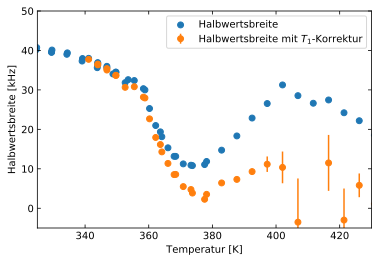
\includegraphics[width=.8\textwidth]{graphics/plot/fwhm_t1.pdf}
	\end{center}
	\caption{Halbwertsbreiten der OBI-Spektren in blau, mit der beschriebenen $T_1$-Korrektur in orange. Die gezeigten Unsicherheiten stammen aus den Unsicherheiten der $T_1$-Werte.} \label{fig:res:spek_fwhm_t1}
\end{figure}

Es ist zu erkennen, dass $T_1$ bei Temperaturen über $\SI{360}{\kelvin}$ einen großen Einfluss auf die Halbwertsbreite hat und die entsprechend angepassten Halbwertsbreiten deutlich geringere Werte aufweisen. Bei Temperaturen über $\SI{410}{\kelvin}$ können auch negative Halbwertsbreiten gefunden werden; diese sind aber aufgrund der hohen Schwankungen der $T_1$-Werte in diesem Temperaturbereich mit entsprechend hohen Unsicherheiten belegt. Eine präzisere Messung von $T_1$ würde eine Korrektur mit geringeren Unsicherheiten erlauben.




Es wurden die am OBI- und am Bruker-Spektrometer aufgenommenen Daten getrennt untersucht, da durch die unterschiedlichen Larmorfrequenzen abweichende Ergebnisse der theoretischen Kurven zu erwarten sind. Bei den Halbwertsbreiten wurde der $T_1$-Einfluss nach der beschriebenen Methode berücksichtigt.



Die aufgenommenen Spektren unterstützen eine biexponentielle Interpretation wie in \eqref{eqn:trans_relax} nur schwerlich, daher wurde lediglich der deutlich zu beobachtende Anteil des Zentralübergangs, $\Delta_c$ und $\omega_c^{(2)}$, für die entsprechenden FWHM- bzw. Schwerpunkts-Daten betrachtet. Für die $T_1$-Daten wird Formel \eqref{eqn:bpp} verwendet. Die Anpassung der Kurven wurde manuell durchgeführt.



Zunächst sollen die Daten des OBI-Spektrometers vergleichen werden. Bei den $T_1$ Werten soll erwähnt werden, dass die Werte bei hohen Temperaturen mit starken Unsicherheiten belegt sind (vlg. Abbildung \ref{fig:res:T_1}) -- entsprechende Indikatoren wurden hier für eine bessere Übersicht ausgelassen.

Für die Spektraldichte $J_\text{BPP}$ kann bei höheren Temperaturen, wie in Abbildung \ref{fig:res:theorie_j} zu sehen, mit dem Parameter $C_Q = \SI{3.6}{MHz}$ eine vergleichsweise gute Übereinstimmung für die Halbwertsbreiten und die Schwerpunkte erreicht werden. Zu tieferen Temperaturen gibt es jedoch gravierende Abweichungen. Für die stark ansteigenden Werte der Halbwertsbreite können anisotrope Effekte vermutet werden, deren Einfluss durch diese isotrope Theorie nicht abgedeckt wird und daher diesen Unterschied kreiert. Gründe für die Abweichungen der Schwerpunkte sind noch offen -- dieser Effekt wird jedoch gleichermaßen in experimentellen als auch simulierten Spektren beobachtet, was bedeutet, dass der Effekt vermutlich auf die von der Simulation berücksichtigten Wechselwirkungen eingeschränkt werden kann.
\begin{figure}
	\begin{center}
		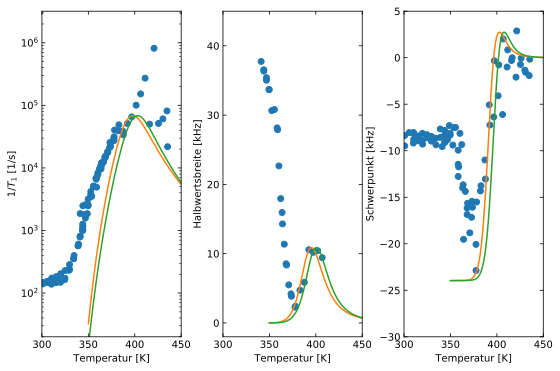
\includegraphics[width=.9\textwidth]{graphics/plot/OBI_J_02.pdf}
	\end{center}
	\caption{Vergleich von $T_1$, Halbwertsbreite und Schwerpunkt der OBI-Daten in blau. In orange die Theorie-Kurve mit Spektraldichte $J_\text{BPP}$ mit Parametern nach \cite{PIMENOV199793}, in grün mit Parametern nach \cite{crn_augsburg}.} \label{fig:res:theorie_j}
\end{figure}

Es kann eine grobe Vereinbarkeit der Theorie mit $T_1$-Werten im Maximum der Kurve erreicht werden, die Flanken unterscheiden sich jedoch deutlich. Da die Form der Theoriekurve mit der Spektraldichte $J_\text{BPP}$ unveränderlich ist, ist es schwerlich möglich, eine zufriedenstellende Übereinstimmung zu erreichen. Abhilfe schaffen könnten andere Spektraldichten -- dies soll im Folgenden untersucht werden.

Für die Spektraldichten $J_\text{CC}$ (Abbildung \ref{fig:res:theorie_j_cc}) und $J_\text{CD}$ (Abbildung \ref{fig:res:theorie_j_dc}) lagen die für die theoretische Berechnung der Schwerpunkte benötigten Imaginärteile $Q_\text{CC}$ und $Q_\text{CD}$ nicht vor, weswegen für diese auf die Spektraldichte $J_\text{BPP}$ zurückgegriffen wurde. Für die Schwerpunkte kann der Vergleich daher nur als grobe Idee verstanden werden.
\begin{figure}
	\begin{center}
		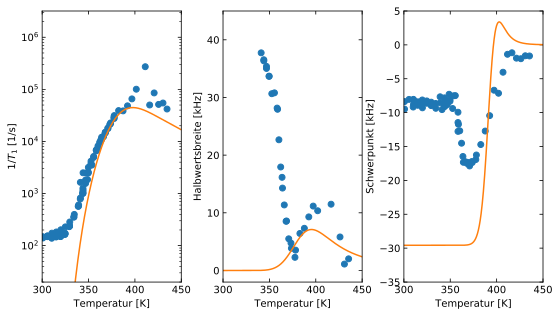
\includegraphics[width=.8\textwidth]{graphics/plot/OBI_J_cc_01.pdf}
	\end{center}
	\caption{Vergleich von $T_1$, Halbwertsbreite und Schwerpunkt der OBI-Daten in blau. In orange die Theoriekurve mit Spektraldichte $J_\text{CC}$ mit Parametern nach \cite{PIMENOV199793}.} \label{fig:res:theorie_j_cc}
\end{figure}
\begin{figure}
	\begin{center}
		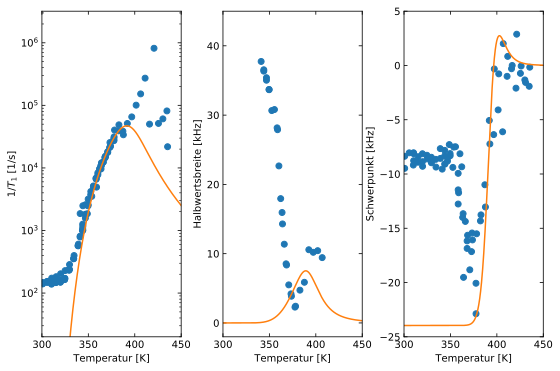
\includegraphics[width=.8\textwidth]{graphics/plot/OBI_J_dc_01.pdf}
	\end{center}
	\caption{Vergleich von $T_1$, Halbwertsbreite und Schwerpunkt der OBI-Daten in blau. In orange die Theorie-Kurve mit Spektraldichte $J_\text{CD}$ mit Parametern nach \cite{PIMENOV199793}.} \label{fig:res:theorie_j_dc}
\end{figure}

Für $J_\text{CC}$ und $J_\text{CD}$ können mit den Parametern $C_Q = \SI{4.0}{MHz}$ und $\alpha = \SI{0.6}{}$ bzw. $C_Q = \SI{3.6}{MHz}$ und $\gamma = \SI{0.46}{}$ gute Übereinstimmungen für $T_1$ beobachtet werden -- zumindest überhalb einer Temperatur von etwa $\SI{350}{\kelvin}$. Für $J_\text{CD}$ scheint es zudem für Temperaturen über $\SI{400}{K}$ Abweichungen zu geben. Bessere Vereinbarkeit mit $T_1$-Werten kommt in beiden Fällen auf Kosten der vergleichsweise guten Übereinstimmungen für Halbwertsbreite und Schwerpunkt, die mit $J_\text{BPP}$ erreicht werden konnten: Während für $J_\text{CC}$ die Schwerpunkte stark abweichen, ist dies bei $J_\text{CD}$ für die Halbwertsbreiten der Fall. Es bleibt festzuhalten, dass insgesamt eine gute Übereinstimmung mit der Theorie gezeigt werden konnte; es kann jedoch keine Spektraldichte besonders vorteilhaft hervorgehoben werden.

Für den Vergleich der Daten des Bruker-Spektrometers ist Ähnliches zu beobachten. Dabei fällt es hier aber schwerer, definitive Aussagen zu treffen, da der eingeschränkte Temperaturbereich nur einen bedingten Vergleich zulässt. Abbildung \ref{fig:res:theorie_bruker} zeigt die Daten zusammen mit Theoriekurven basierend auf der Spektraldichte $J_\text{BPP}$ mit dem Parameter $C_Q = \SI{3.45}{MHz}$. Dabei ist zu sehen, dass die Daten im gleichen Maße wie die OBI-Daten Übereinstimmungen und Unterschiede aufzeigen.
\begin{figure}
	\begin{center}
		\includegraphics[width=.9\textwidth]{graphics/plot/Bruker_J_01.pdf}
	\end{center}
	\caption{Vergleich von $T_1$, Halbwertsbreite und Schwerpunkt der Bruker-Daten in blau. In orange die Theorie-Kurve mit Spektraldichte $J_\text{BPP}$ mit Parametern nach \cite{PIMENOV199793}.} \label{fig:res:theorie_bruker}
\end{figure}



\chapter{Zusammenfassung und Ausblick}

Ein Ziel dieser Arbeit war es, im Temperaturbereich um und unter der Glasübergangstemperatur von $T_g = \SI{333}{K}$ von Calciumrubidiumnitrat, oder CRN, mit der $^\text{87}$Rb-NMR nach Hinweisen auf ionische Dynamik zu suchen. Dafür wurden sowohl stimulierte Echos als auch die Breiten pulsabstandsahängiger Spektren aufgenommen und analysiert. Es wurde erwartet, dass die Zeitskalen der gefundenen Zeitkonstanten die Existenz eine Betaprozesses, wie sie Abbildung \ref{fig:einl:zuernpaper} andeutet, unterstützen. Dies konnte jedoch nicht bestätigt werden -- die gefunden Zeitkonstanten liegen mehrere Größenordnungen über den Erwartungen. Eine mögliche Erklärung wäre, dass die Stoffe CRN und CKN in diesem Bereich unterschiedliche Eigenschaften aufweisen und der Betaprozesses tatsächlich nur für CKN erwartet werden kann. Dies ist aber aufgrund der Ähnlichkeit der Stoffe in anderen Eigenschaften eher unwahrscheinlich. Eine Klärung könnte durch Untersuchungen mit anderen spektroskopischen Methoden versucht werden.

Desweiteren wurde eine Untersuchung der Linienformänderung von CRN-Spektren im Verlauf der Temperatur durchgeführt. Dazu wurden sowohl experimentelle Spektren an zwei Spektrometern mit unterschiedlicher Larmorfrequenz aufgenommen, als auch Simulationen auf Basis eines isotropen Sprungs mit einer Czjzek-Verteilung als Ausgangspunkt durchgeführt. Im Temperaturbereich unter $\SI{375}{K}$ weisen Simulation und Experimente eine gute Übereinstimmung der Linienform auf; zu höheren Temperaturen sind starke Abweichungen zu beobachten. Hier könnten die Erkenntnisse, die beim Vergleich von experimentellen Spektren und Theorie gewonnen wurden, helfen, um über den ganzen Temperaturbereich eine zufriedenstellende Übereinstimmung zu erreichen.

Zu dem hier verwendeten Czjzek-Modell mit isotropem Sprung wurde ergänzend ein Oktaeder-Modell vorgeschlagen. Dieses kann bestimmte, in diesem Kontext erwünschte, Eigenschaften wie die Czjzek-Linienform replizieren, erlaubt jedoch deutlich feinere Anpassungen des Bewegungsmodells. Während die Anfänge dieses Modells vielversprechend scheinen, ist mehr Arbeit notwendig, um es zum Einsatz zu bringen und daraus Erkenntnisse zu gewinnen.

Die experimentellen Spektren sind im Bezug auf die unterschiedlichen verwendeten Larmorfrequenzen in sich konsistent, zeigen jedoch sowohl bei der Halbwertsbreite als auch bei den Schwerpunkten der Spektren leichte Unterschiede. Messungen an weiteren Spektrometern mit zusätzlichen Larmorfrequenzen könnten helfen, die Einflüsse von chemischer Verschiebung und Quadrupol-Wechselwirkung zweiter Ordnung zu trennen und aufzuschlüsseln. 

Die experimentellen Spektren wurden zudem mit der Theorie der Quadrupol-Wech\-sel\-wir\-kung zweiter Ordnung verglichen. Dazu wurden die experimentell gemessenen Werte für $T_1$ sowie die Halbwertsbreiten und Schwerpunkte von Spektren mit den von der Theorie vorhergesagten verglichen. Dabei wurden für unterschiedliche verwendete Spektraldichten unterschiedliche Übereinstimmungen gefunden. Die Spektraldichte $J_\text{BPP}$ zeigt für Temperaturen über $\SI{375}{K}$ gute Deckungen mit der Halbwertsbreite und den Schwerpunkten der experimentellen Spektren, aber deutliche Abweichungen bei $T_1$. Die Spektraldichten $J_\text{CC}$ und $J_\text{CD}$ zeigten das umgekehrte Verhalten: Während für Temperaturen über $\SI{350}{K}$ besonders mit $J_\text{CC}$ eine gute Übereinstimmung zu $T_1$ erreicht werden konnte, gibt es hier für die Halbwertsbreiten und Schwerpunkte größere Abweichungen. Keine der verwendeten Spektraldichten konnte mit einem Parametersatz eine Deckung für $T_1$, die Halbwertsbreiten und die Schwerpunkte erreichen. Zur Klärung der Gründe hierfür sind weitere Untersuchungen notwendig. Messungen zu höheren Temperaturen, beispielsweise mit dem Hochtemperatur-Probenkopf, könnten bestimmen, inwiefern die Experimente auch in anderen als den hier untersuchen Temperaturbereichen mit der Theorie konsistent sind.

% Der Einfluss eines kurzen $T_1$ bei Temperaturen über $\SI{370}{K}$ konnte in der Halbwertsbreite beobachtet, und, für einen besseren Vergleich mit der Theorie, rechnerisch eliminiert werden.



\printbibliography

\appendix
% Hier beginnt der Anhang, nummeriert in lateinischen Buchstaben
% \input{content/a_tensorundwignerd.tex}
% \input{content/b_qww2gedreht.tex}
% \input{content/c_pulsprogrammbruker.tex}


\backmatter


\cleardoublepage
\input{content/eid_versicherung.tex}
\end{document}
